\documentclass[10pt]{IEEEtran}
\usepackage[utf8]{inputenc}
\usepackage{graphicx}
\usepackage{float}
\bibliographystyle{ieeetr}

\title{Multiprocesamiento en Multiplicacion de Matrices}
\author{
  \IEEEauthorblockN{Blancarte Lopez Jorge,
  Barrera Oropeza Jose Antonio,
  Carrera Sanchez Martha Elena,
  Lievana Poy Erick and
  Lopez Aguilar Eduardo}\\
  \IEEEauthorblockA{Facultad de Ciencias de la Computación,
  Benemérita Universidad Autónoma de Puebla
  Email:jorge.blancarte@alumno.buap.mx,
  jose.barrerao@alumno.buap.mx,
  martha.carrera@alumno.buap.mx,
  erick.lievanap@alumno.buap.mx,
  eduardo.lopezg@alumno.buap.mx}}

\begin{document}

\maketitle

\begin{abstract}
  El reporte presentado trata acerca de la aplicación y de un escenario multiprocesamiento para comparar un algoritmo paralelo de multiplicación de matrices, el Algoritmo de Fox y Multiplicación de matrices con un algoritmo secuencial, ambos algoritmos se desarrollaron utilizando la librería MPI y OpenMP.
\end{abstract}

\begin{IEEEkeywords}
  Algoritmo, Paralelo, Secuencial, Tiempo, Memoria, Fox OMP, Fox MPI.
\end{IEEEkeywords}

\section{Introducción}
Para el presente artículo tiene por objetivo aplicar y crear un escenario comparativo de dos versiones de algoritmos de multiplicación de matrices con diferentes mecanismos y particionamiento de tareas, en particular los algoritmos de Fox y de multiplicación con un algoritmo secuencial. Posteriormente se desea comparar el comportamiento de los mismos con diferentes cargas de trabajo  y comparar su desempeño con la versión en un core, dos cores, tres cores y cuatro cores mas. Para el desarrollo de las versiones en paralelo se ha utilizado la librería de paso de mensajes MPI y OpenMP con el compilador gcc.Se describirá cada una de las implementaciones desarrolladas.

\section{Antecedentes}

\subsection{Algoritmo de Fox}
Este algoritmo está orientado a las máquinas paralelas de memoria distribuida y se puede explicar en términos del modelo de cómputo paralelo SPMD junto con la distribución de los datos de las matrices.

Para realizar la multiplicación se utilizan p tareas o procesos ubicados sobre una grilla de m$\times$m elementos, siendo $p= m^2$ Cada tarea calculará un bloque de n$\times$n elementos de la matriz resultado. El tamaño de las matrices A, B y C es (n$\times$m)(n$\times$m), es decir que se opera con matrices cuadradas de orden N = (n$\times$m). Las matrices A, B y C son almacenadas como bloques distribuidos en las $m^2$ tareas. Cada tarea tij (donde i es la fila y j es la columna de la grilla de procesadores) contiene los bloques Aij, Bij y Cij.

\begin{figure}[H]
  \centering
  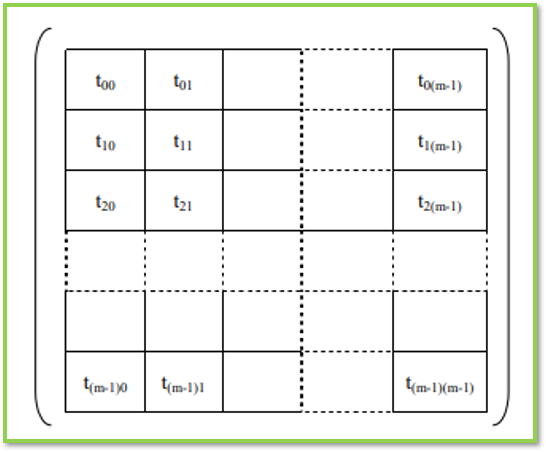
\includegraphics[width=.9\linewidth]{figs/matrizfox.png}
  \caption{Muestra una matriz dividida en bloques y su distribución entre las distintas tareas. Esta distribución es igual para las tres matrices (A, B y C).}
  \label{fig:example}
\end{figure}

\subsection{MPI}
MPI (iniciales de Message Passing Interface) es una especificación para programación de paso de mensajes, que proporciona una librer´ıa de funciones para C, C++ y Fortran que son empleadas en los programas para comunicar datos y portable, especificada por consenso por el MPI Forum, con unas 40 organizaciones participantes, como modelo que permita desarrollar programas que puedan ser migrados a diferentes computadores paralelos.

Definido conjuntamente por proveedores de hardware y de software, OpenMP es un modelo de programación portable y escalable que proporciona a los programadores una interfaz simple y flexible para el desarrollo de aplicaciones paralelas, para plataformas que van desde las computadoras de escritorio hasta supercomputadoras.

\subsection{OMP}
OpenMP es una interfaz de programación de aplicaciones (API) para la programación multiproceso de memoria compartida en múltiples plataformas. Permite añadir concurrencia a los programas escritos en C, C++ y Fortran sobre la base del modelo de ejecución fork-join. Está disponible en muchas arquitecturas, incluidas las plataformas de Unix y de Microsoft Windows. Se compone de un conjunto de directivas de compilador, rutinas de biblioteca, y variables de entorno que influyen el comportamiento en tiempo de ejecución.

Definido conjuntamente por proveedores de hardware y de software, OpenMP es un modelo de programación portable y escalable que proporciona a los programadores una interfaz simple y flexible para el desarrollo de aplicaciones paralelas, para plataformas que van desde las computadoras de escritorio hasta supercomputadoras. Una aplicación construida con un modelo de programación paralela híbrido se puede ejecutar en un cluster de computadoras utilizando OpenMP y MPI, o a través de las extensiones de OpenMP para los sistemas de memoria distribuida.

\subsection{Gnuplot}
Gnuplot es un programa en línea de comandos que permite dibujar gráficas de funciones en 2 y 3 dimensiones a través de las fórmulas que las definen. También puede dibujar gráficos usando una tabla de coordenadas (en formato sólo texto) creadas con cualquier programa.

El software tiene copyright pero se distribuye libremente y está disponible para UNIX, Linux, IBM OS/2, MS Windows, MSDOS, Macintosh, VMS, Atari y muchas otras plataformas.

\begin{figure}[H]
  \centering
  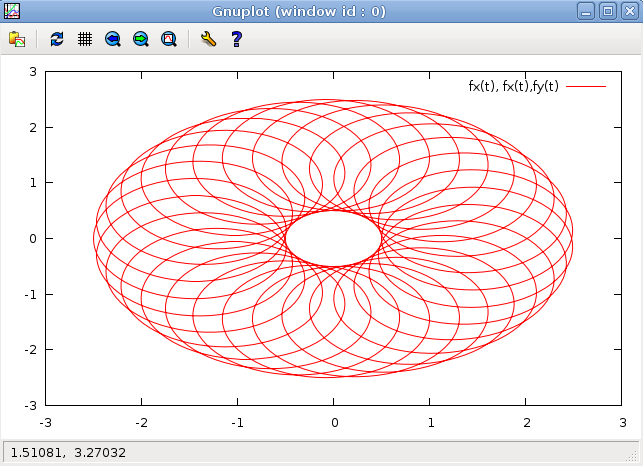
\includegraphics[width=.9\linewidth]{figs/gnuplot3.png}
  \caption{Una gráfica en Gnuplot.}
  \label{fig:gnuplot}
\end{figure}

\subsubsection{Características}
\begin{itemize}
  \item Representaciones bidimensionales con distintos estilos como puntos, líneas, barras.
  \item Representaciones tridimensionales (contorno y superficie).
  \item Facilidades para etiquetar las gráficas, ejes y puntos representados (títulos y etiquetas).
  \item Permite realizar cálculos con enteros, decimales y complejos.
  \item Capacidad de guardar y exportar todos los comandos que hayamos utilizado para generar una gráfica.
  \item Exportar un script con una serie de comandos desde una macro; y la generación de un código en \LaTeX{} de las gráficas hechas
\end{itemize}

\section{Desarrollo}
Para este trabajo se desarrollaron 2 implementaciones del algoritmo paralelo Fox, una hecha en MPI y otra hecha en OMP. Asi mismo se hizo una implementacion del algoritmo secuencial de multiplicación de matrices. Todas las implementaciones fueron hechas en el lenguaje de programación C.

Se realizaron 100 ejecuciones para cada tipo de matrices, las categorias son:
\begin{itemize}
  \item Tipo de dato: short, int, float, double
  \item Orden de matriz: 64, 128, 256, 512, 1024, 2048
  \item Numero de cores: 1 core y 4 core
\end{itemize}

Se tomaron mediciones del uso de memoria y el tiempo de ejecución de cada multiplicación de matrices. Estas matrices se llenan con valores densos y pseudoaleatorios de números reales de 1000 a 2000.

\subsection{Descripción del Hardware}

Estas pruebas se ejecutaron en las siguientes computadoras.

\textbf{Caracteristicas de computadora 1:}
\begin{itemize}
  \item Procesador: Intel(R) Core(TM) i7-7700K CPU @ 4.20GHz
  \item Memoria: 16GB RAM
  \item Disco Duro: 500 GB
  \item S.O: ArchLinux
  \item Thread(s) por core: 2
  \item Core(s) por socket: 4
\end{itemize}

\textbf{Caracteristicas de computadora 2:}
\begin{itemize}
  \item Procesador: Intel(R) Core(TM) i5-1035G1 CPU @ 1.00GHz
  \item Memoria: 12GB RAM
  \item Disco Duro: 500 GB
  \item S.O:  Ubuntu
  \item Thread(s) por core: 2
  \item Core(s) por socket: 4
\end{itemize}

\subsection{Algoritmo de forma secuencial}

Para su solución se emplea una serie de acciones ejecutadas constantemente en un órden secuencial. Las tareas se ejecutan una tras otra a modo de secuencia, es decir que una instrucción no se ejecuta hasta que finaliza la anterior. Dentro de este tipo podemos encontrar operaciones de inicio/fin, inicialización de variables, operaciones de asignación, cálculo, sumarización. Los algoritmos que necesitan de estructuras secuenciales para su solución son los mas difíciles de comprender y mas sencillos de identificar los procesos que realizará el programa que nos llevarán a la solución del mismo.

Este tipo de estructura se basa en las 5 fases que consta todo algoritmo:

\begin{itemize}
  \item Definición de variables (Declaración).
  \item Inicialización de variables.
  \item Lectura de datos.
  \item Cálculos.
  \item Salida.
\end{itemize}

\section{Resultados}

Para el análisis de los datos obtenidos se decidio comparar la eficiencia de los algoritmos en los distintos tipos de datos, comparando su ejecución en 1 y 4 cores.

\subsection{Datos Short}

\subsection{Resultados con un nucleo}

\begin{figure}[H]
  \centering
  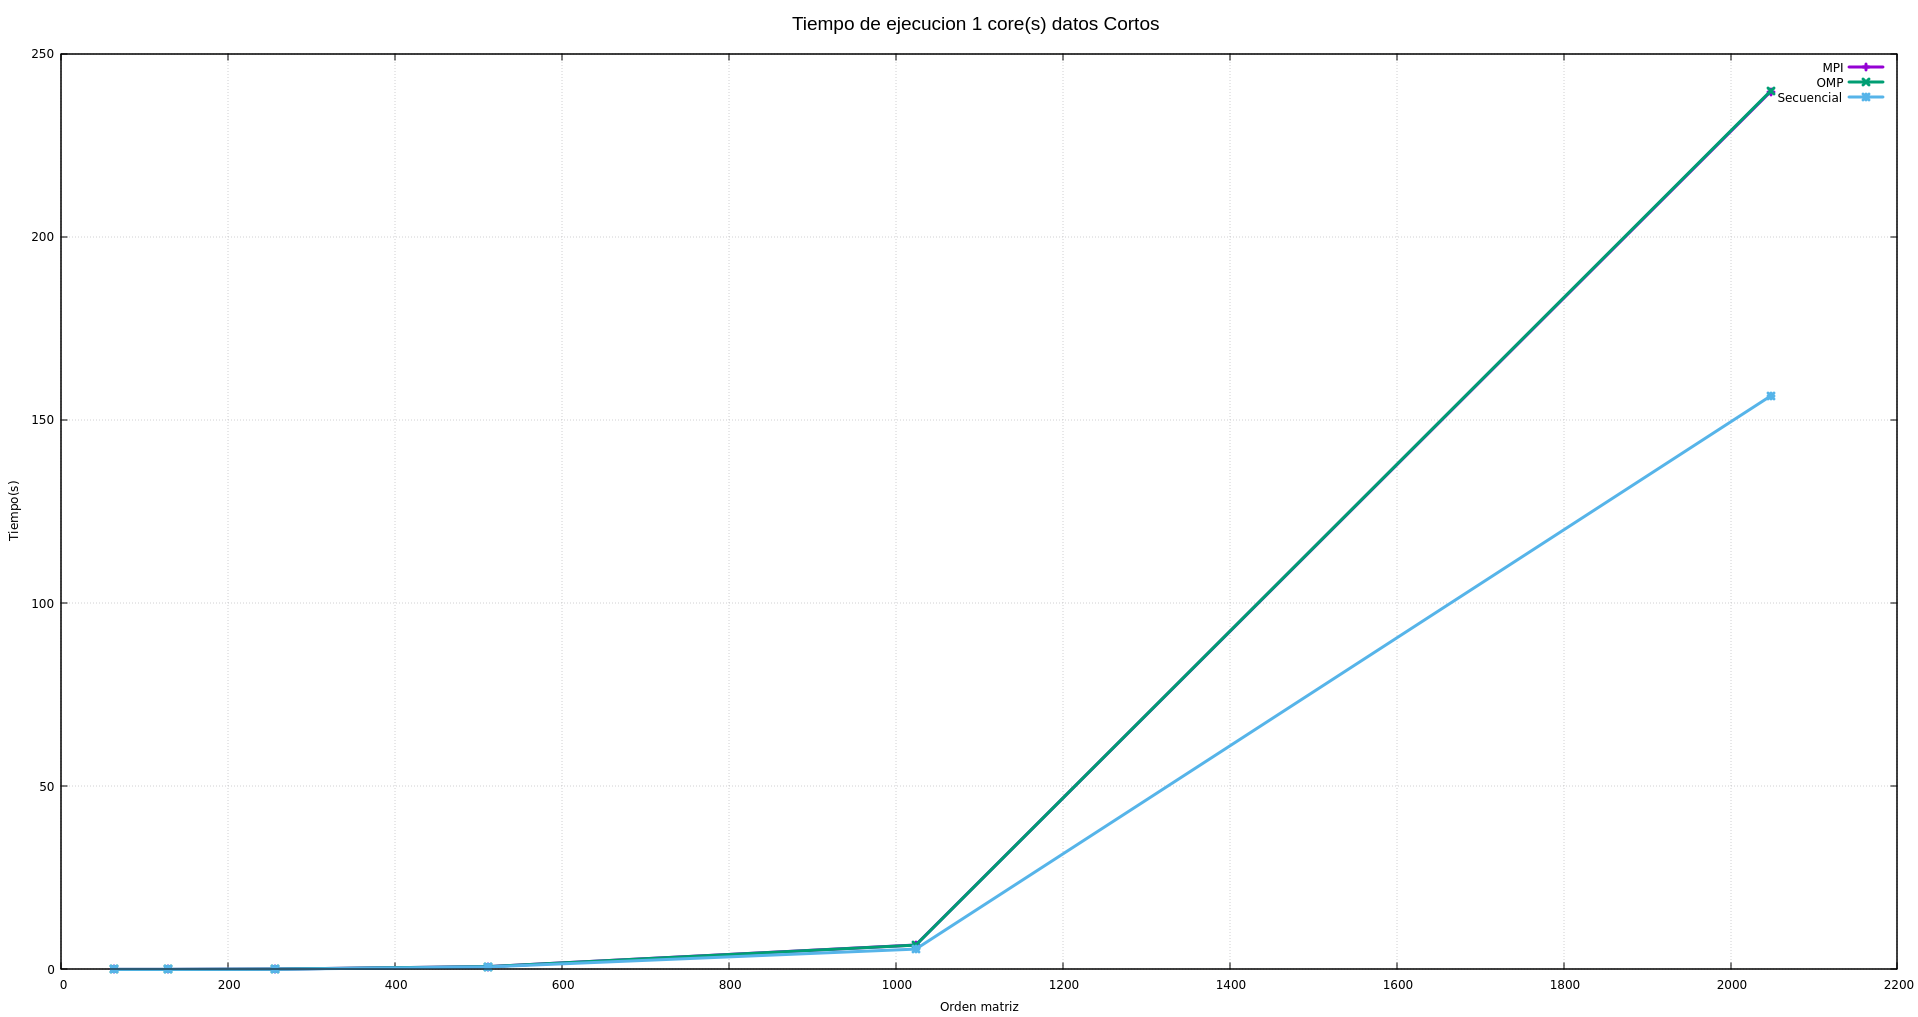
\includegraphics[width=0.95\linewidth]{figs/1nucleoCortosTiempo.png}
  \caption{Tiempo de ejecución datos Short 1 nucleo}
  \label{fig:cor}
\end{figure}

\begin{table}[H]
  \caption{Tiempo de ejecución datos Short 1 nucleo}
  \label{table_example}
  \centering
  \begin{tabular}{|c|c|c|c|}
    \hline
    \textbf{Orden} & \textbf{MPI} & \textbf{OMP} & \textbf{Secuencial} \\
    \hline
    64 & 0.001426 & 0.001269 & 0.000921 \\
    128 & 0.011359 & 0.010856 & 0.007884 \\
    256 & 0.070067 & 0.069140 & 0.065247 \\
    512 & 0.754682 & 0.758296 & 0.691954 \\
    1024 & 6.654911 & 6.619214 & 5.544929 \\
    2048 & 239.580876 & 239.742824 & 156.494765 \\
    \hline
  \end{tabular}
\end{table}

\begin{figure}[H]
  \centering
  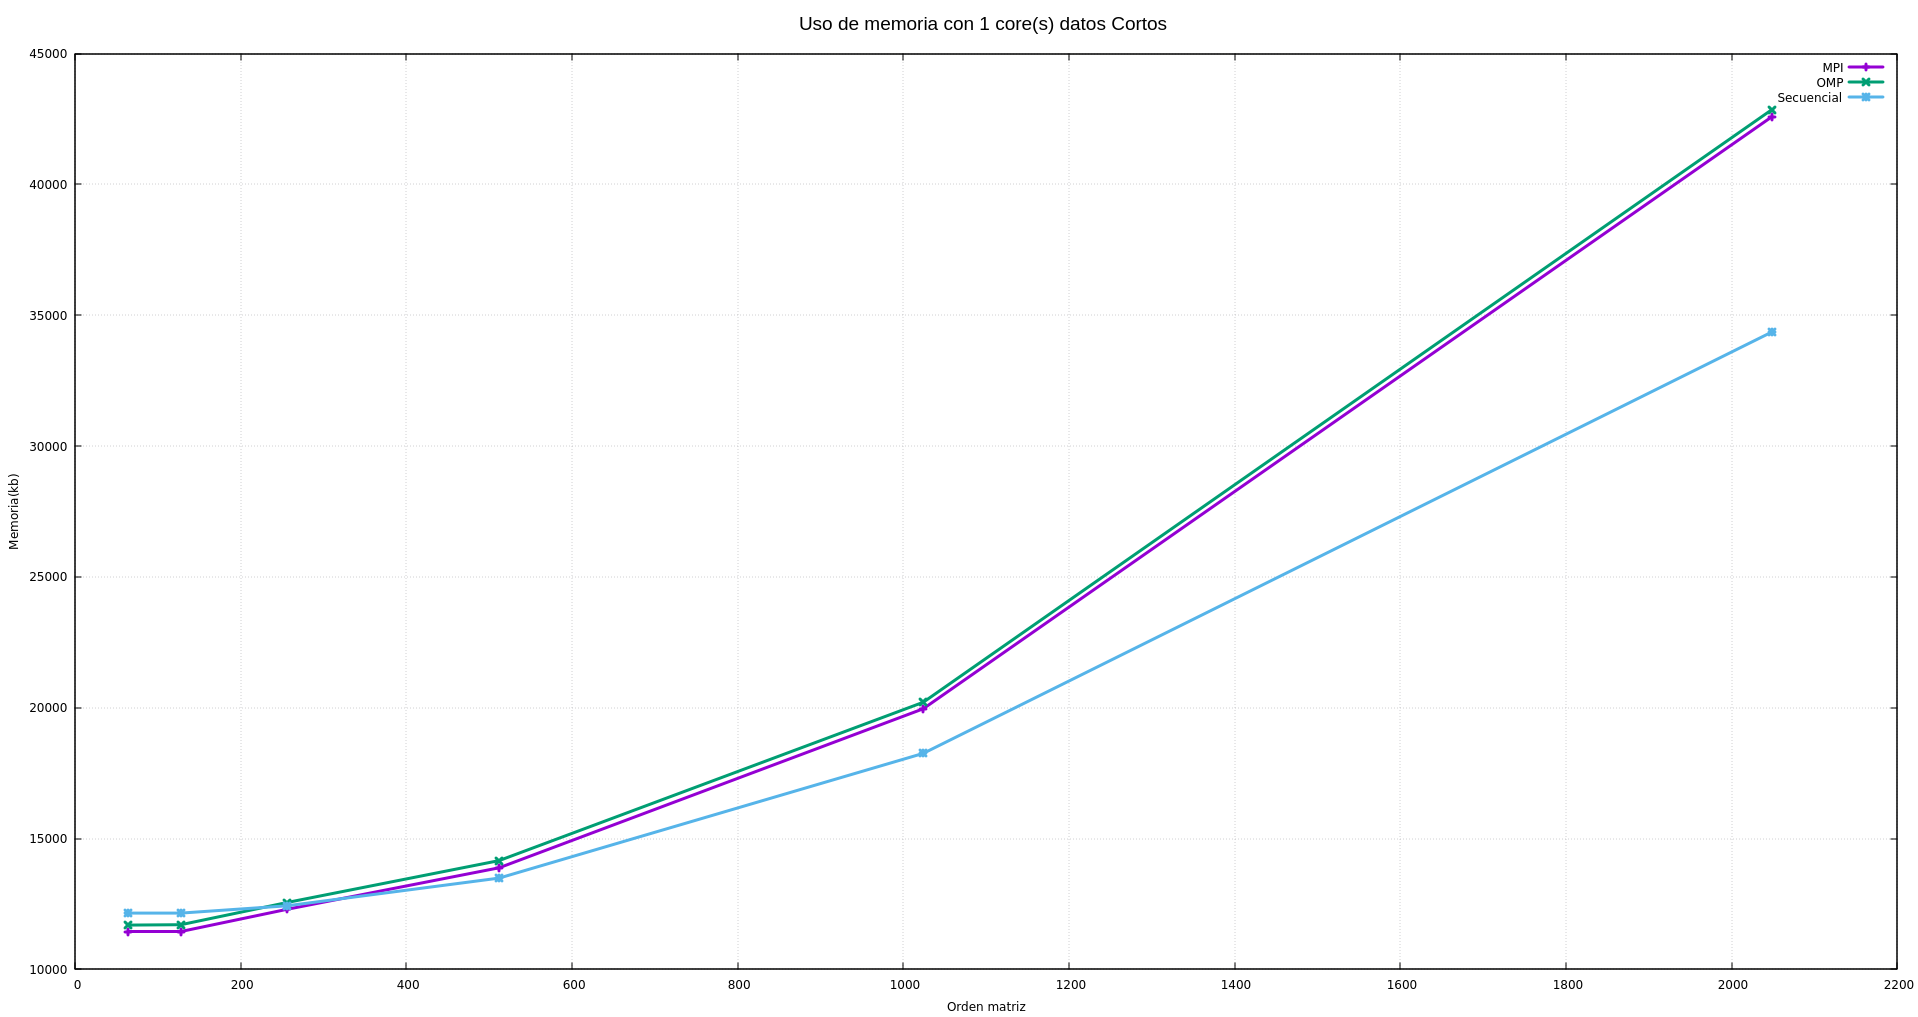
\includegraphics[width=0.95\linewidth]{figs/1nucleoCortosMemoria.png}
  \caption{Uso de memoria(kb) datos Short 1 cores}
  \label{fig:cor2}
\end{figure}

\begin{table}[H]
  \caption{Uso de memoria(kb) datos Short 1 cores}
  \label{table_example}
  \centering
  \begin{tabular}{|c|c|c|c|}
    \hline
    \textbf{Orden} & \textbf{MPI} & \textbf{OMP} & \textbf{Secuencial} \\
    \hline
    64 & 11449.760000 & 11693.160000 & 12149.720000 \\
    128 & 11447.800000 & 11708.920000 & 12150.600000 \\
    256 & 12297.520000 & 12557.880000 & 12428.600000 \\
    512 & 13882.040000 & 14156.280000 & 13490.240000 \\
    1024 & 19959.680000 & 20207.680000 & 18254.880000 \\
    2048 & 42574.120000 & 42846.440000 & 34351.680000 \\
    \hline
  \end{tabular}
\end{table}

\subsection{Resultados con 4 nucleos}

\begin{figure}[H]
  \centering
  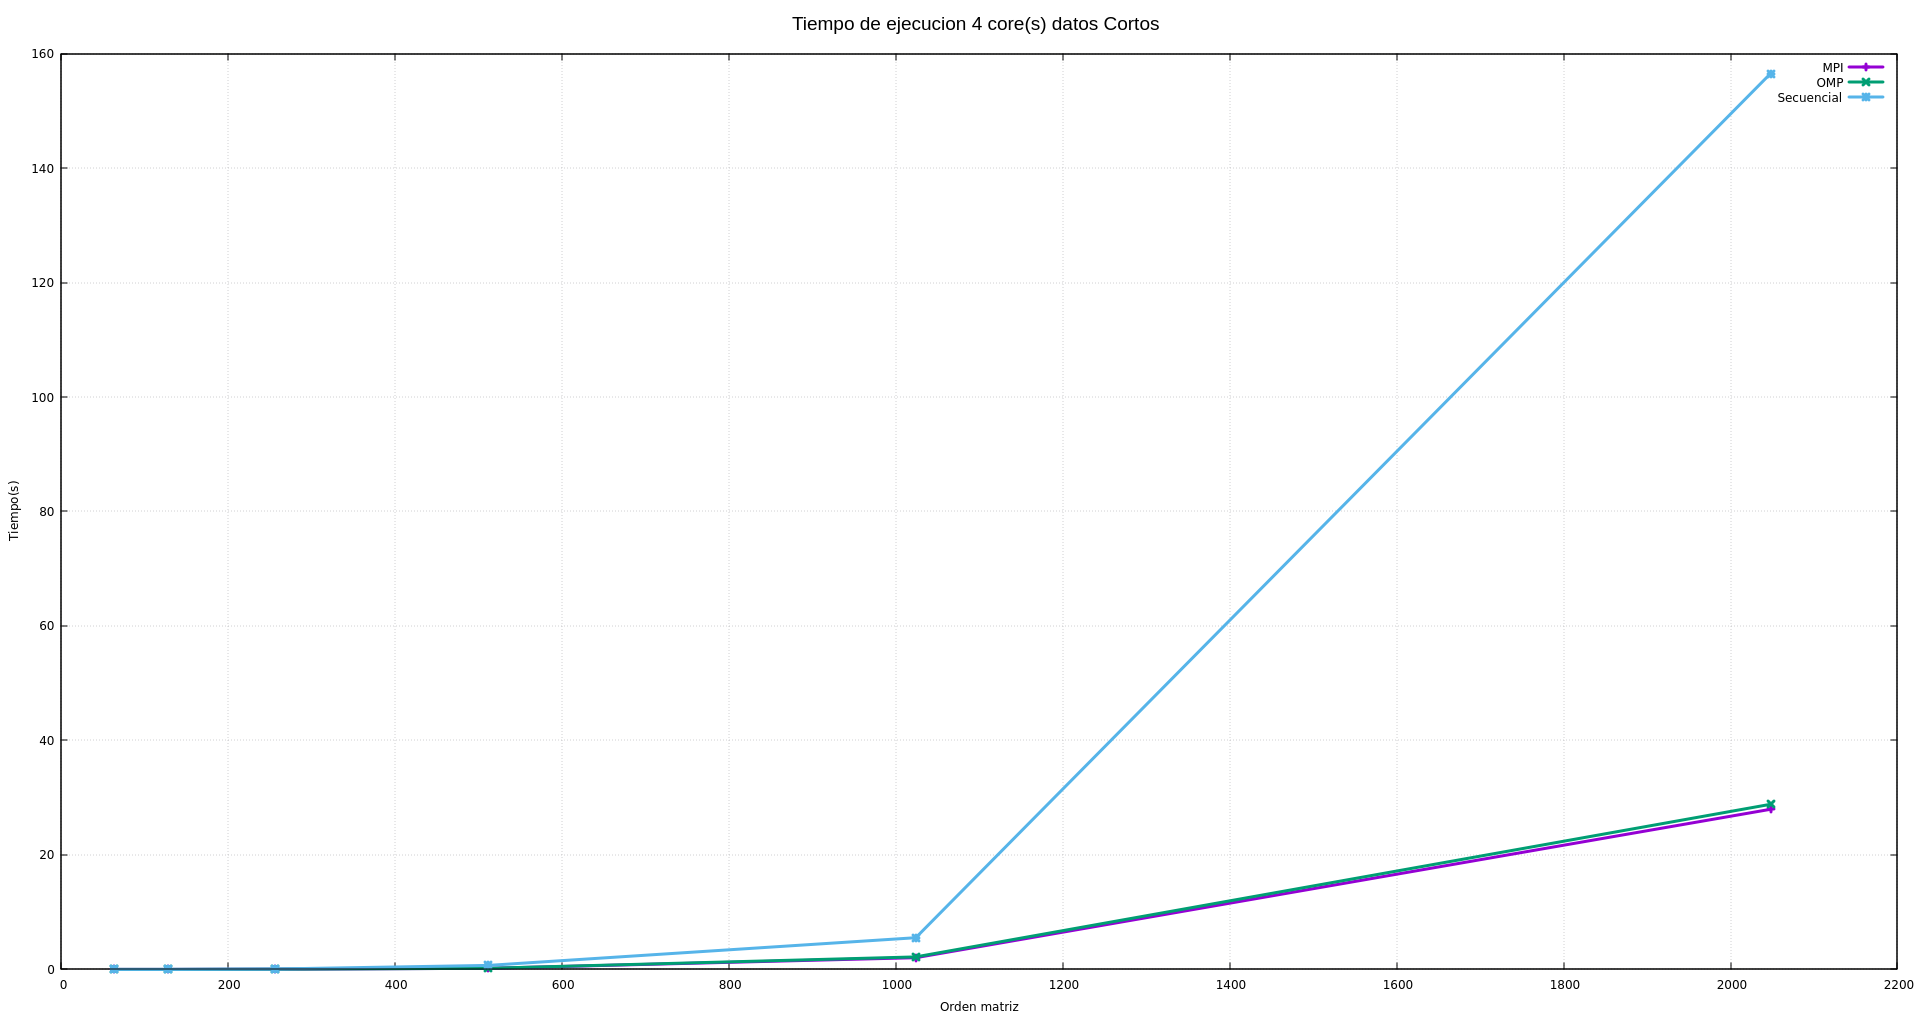
\includegraphics[width=0.95\linewidth]{figs/4nucleosCortosTiempo.png}
  \caption{Tiempo de ejecución datos Short 4 nucleo}
  \label{fig:c}
\end{figure}

\begin{table}[H]
  \caption{Tiempo de ejecución datos Short 4 nucleo}
  \label{table_example}
  \centering
  \begin{tabular}{|c|c|c|c|}
    \hline
    \textbf{Orden} & \textbf{MPI} & \textbf{OMP} & \textbf{Secuencial} \\
    \hline
    64 & 0.000764 & 0.000706 & 0.000921 \\
    128 & 0.004566 & 0.004693 & 0.007884 \\
    256 & 0.034549 & 0.034827 & 0.065247 \\
    512 & 0.196879 & 0.199415 & 0.691954 \\
    1024 & 2.040931 & 2.180215 & 5.544929 \\
    2048 & 27.964720 & 28.835194 & 156.494765 \\
    \hline
  \end{tabular}
\end{table}

\begin{figure}[H]
  \centering
  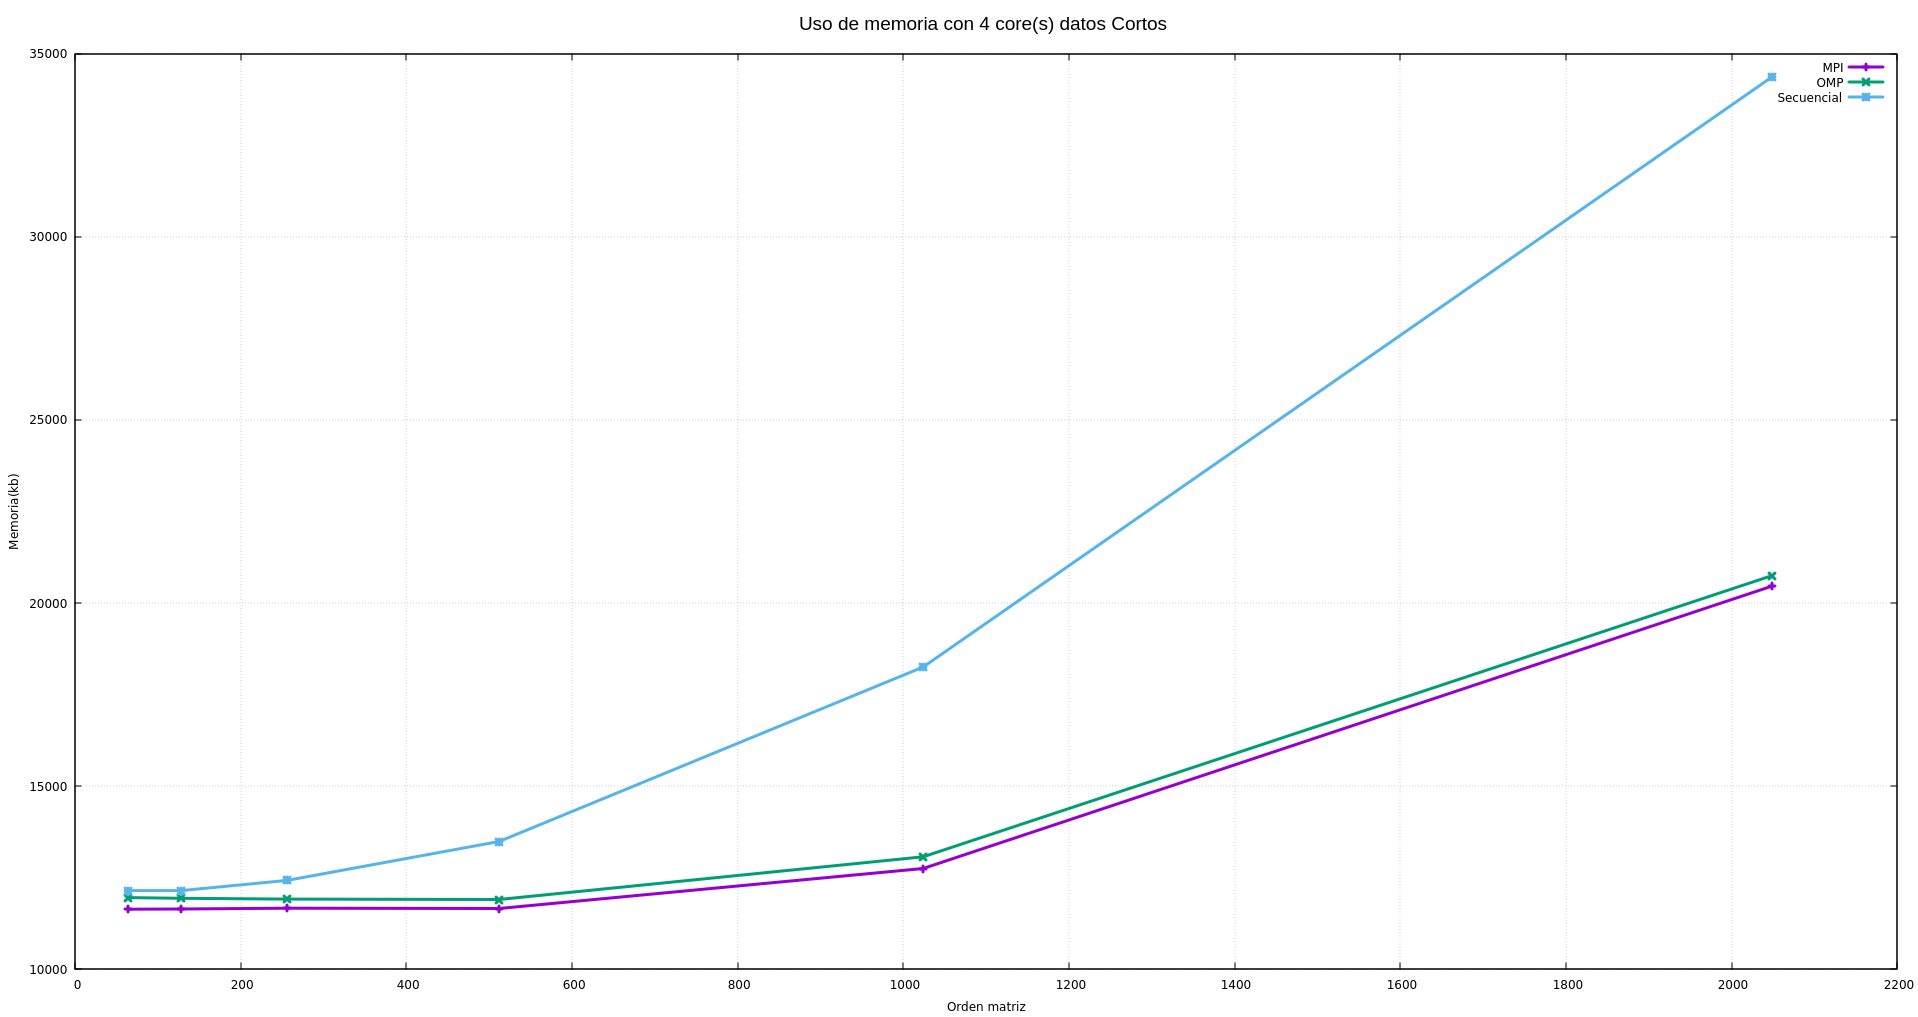
\includegraphics[width=0.95\linewidth]{figs/4nucleosCortosMemoria.png}
  \caption{Uso de memoria(kb) datos Short 4 cores}
  \label{fig:c2}
\end{figure}

\begin{table}[H]
  \caption{Uso de memoria(kb) datos Short 4 cores}
  \label{table_example}
  \centering
  \begin{tabular}{|c|c|c|c|}
    \hline
    \textbf{Orden} & \textbf{MPI} & \textbf{OMP} & \textbf{Secuencial} \\
    \hline
    64 & 11642.320000 & 11959.360000 & 12149.720000 \\
    128 & 11648.800000 & 11941.200000 & 12150.600000 \\
    256 & 11670.720000 & 11918.840000 & 12428.600000 \\
    512 & 11663.640000 & 11909.280000 & 13490.240000 \\
    1024 & 12752.960000 & 13073.960000 & 18254.880000 \\
    2048 & 20457.720000 & 20744.160000 & 34351.680000 \\
    \hline
  \end{tabular}
\end{table}

\subsection{Datos Int}

\subsection{Resultados con un nucleo}

\begin{figure}[H]
  \centering
  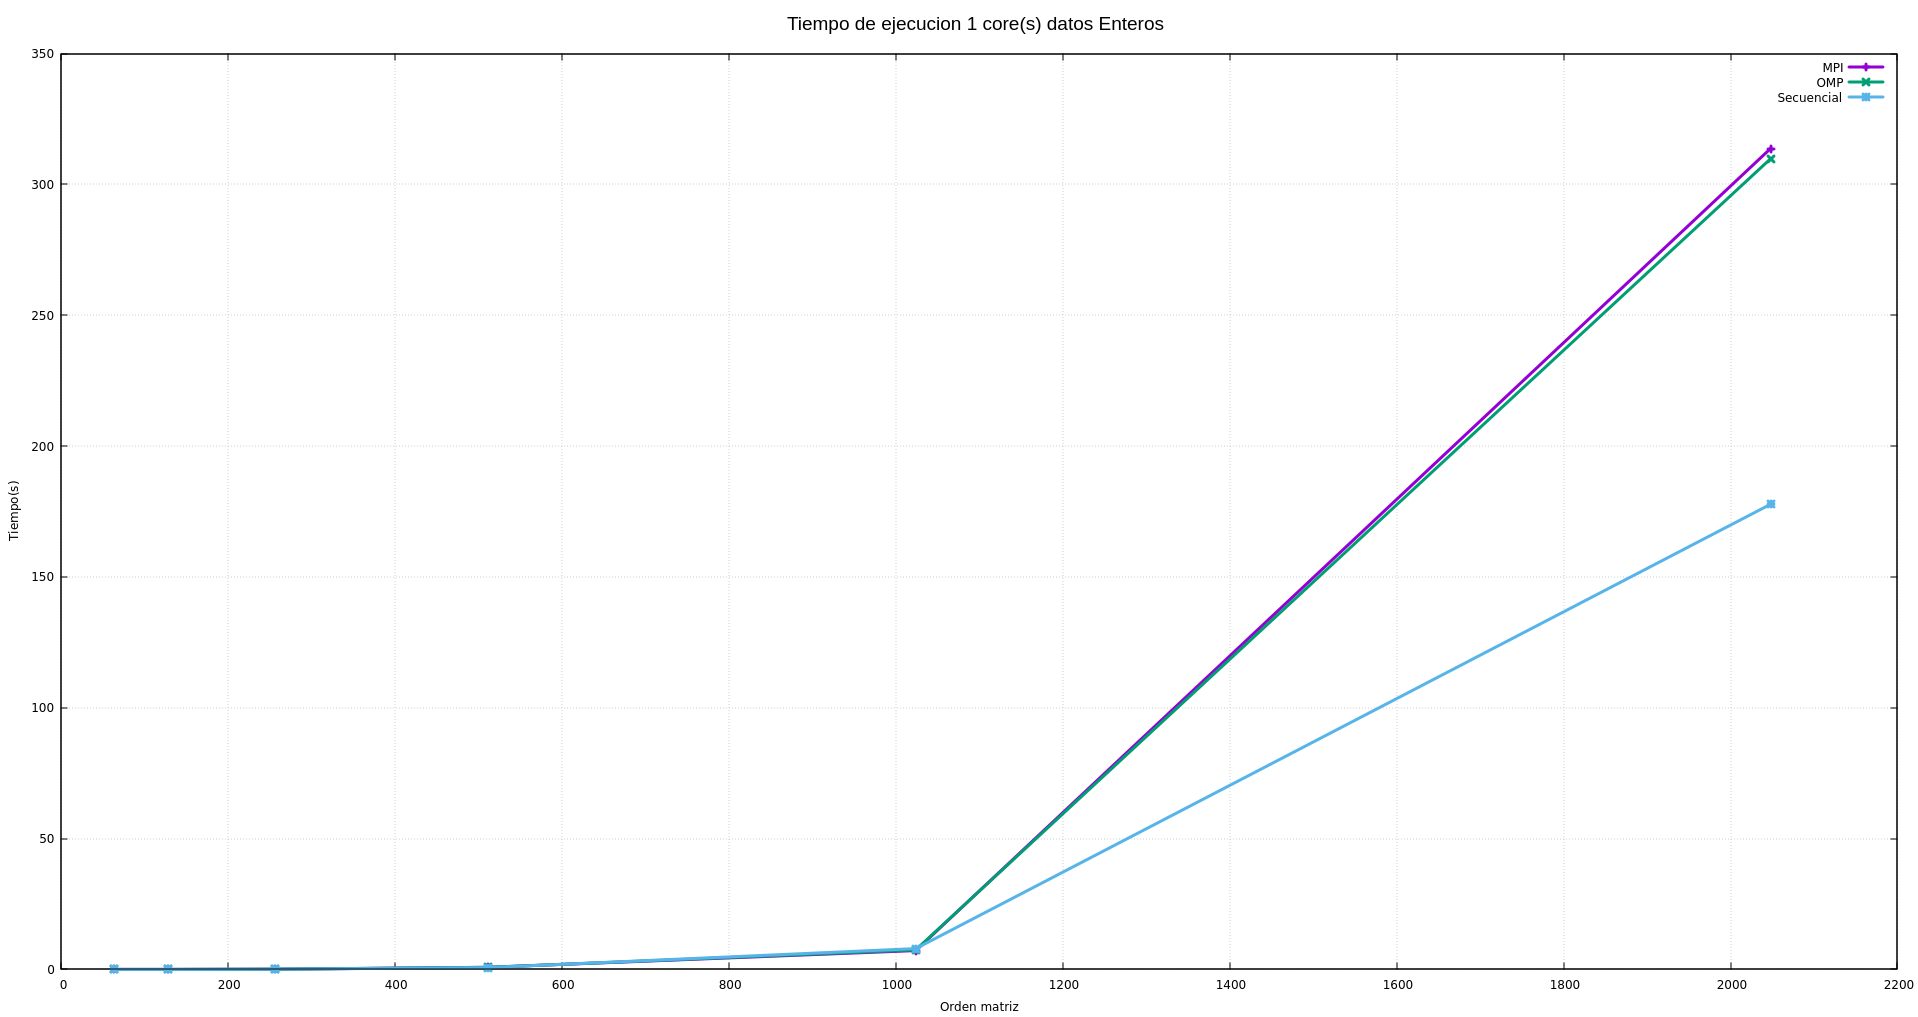
\includegraphics[width=0.95\linewidth]{figs/1nucleoEnterosTiempo.png}
  \caption{Tiempo de ejecución datos Int 1 nucleo}
  \label{fig:int}
\end{figure}

\begin{table}[H]
  \caption{Tiempo de ejecución datos Int 1 nucleo}
  \label{table_example}
  \centering
  \begin{tabular}{|c|c|c|c|}
    \hline
    \textbf{Orden} & \textbf{MPI} & \textbf{OMP} & \textbf{Secuencial} \\
    \hline
    64 & 0.001319 & 0.001369 & 0.000924 \\
    128 & 0.011740 & 0.011952 & 0.008235 \\
    256 & 0.082202 & 0.081473 & 0.080314 \\
    512 & 0.812428 & 0.809918 & 0.693803 \\
    1024 & 7.185841 & 7.463824 & 7.939406 \\
    2048 & 313.668473 & 309.743006 & 177.748948 \\
    \hline
  \end{tabular}
\end{table}

\begin{figure}[H]
  \centering
  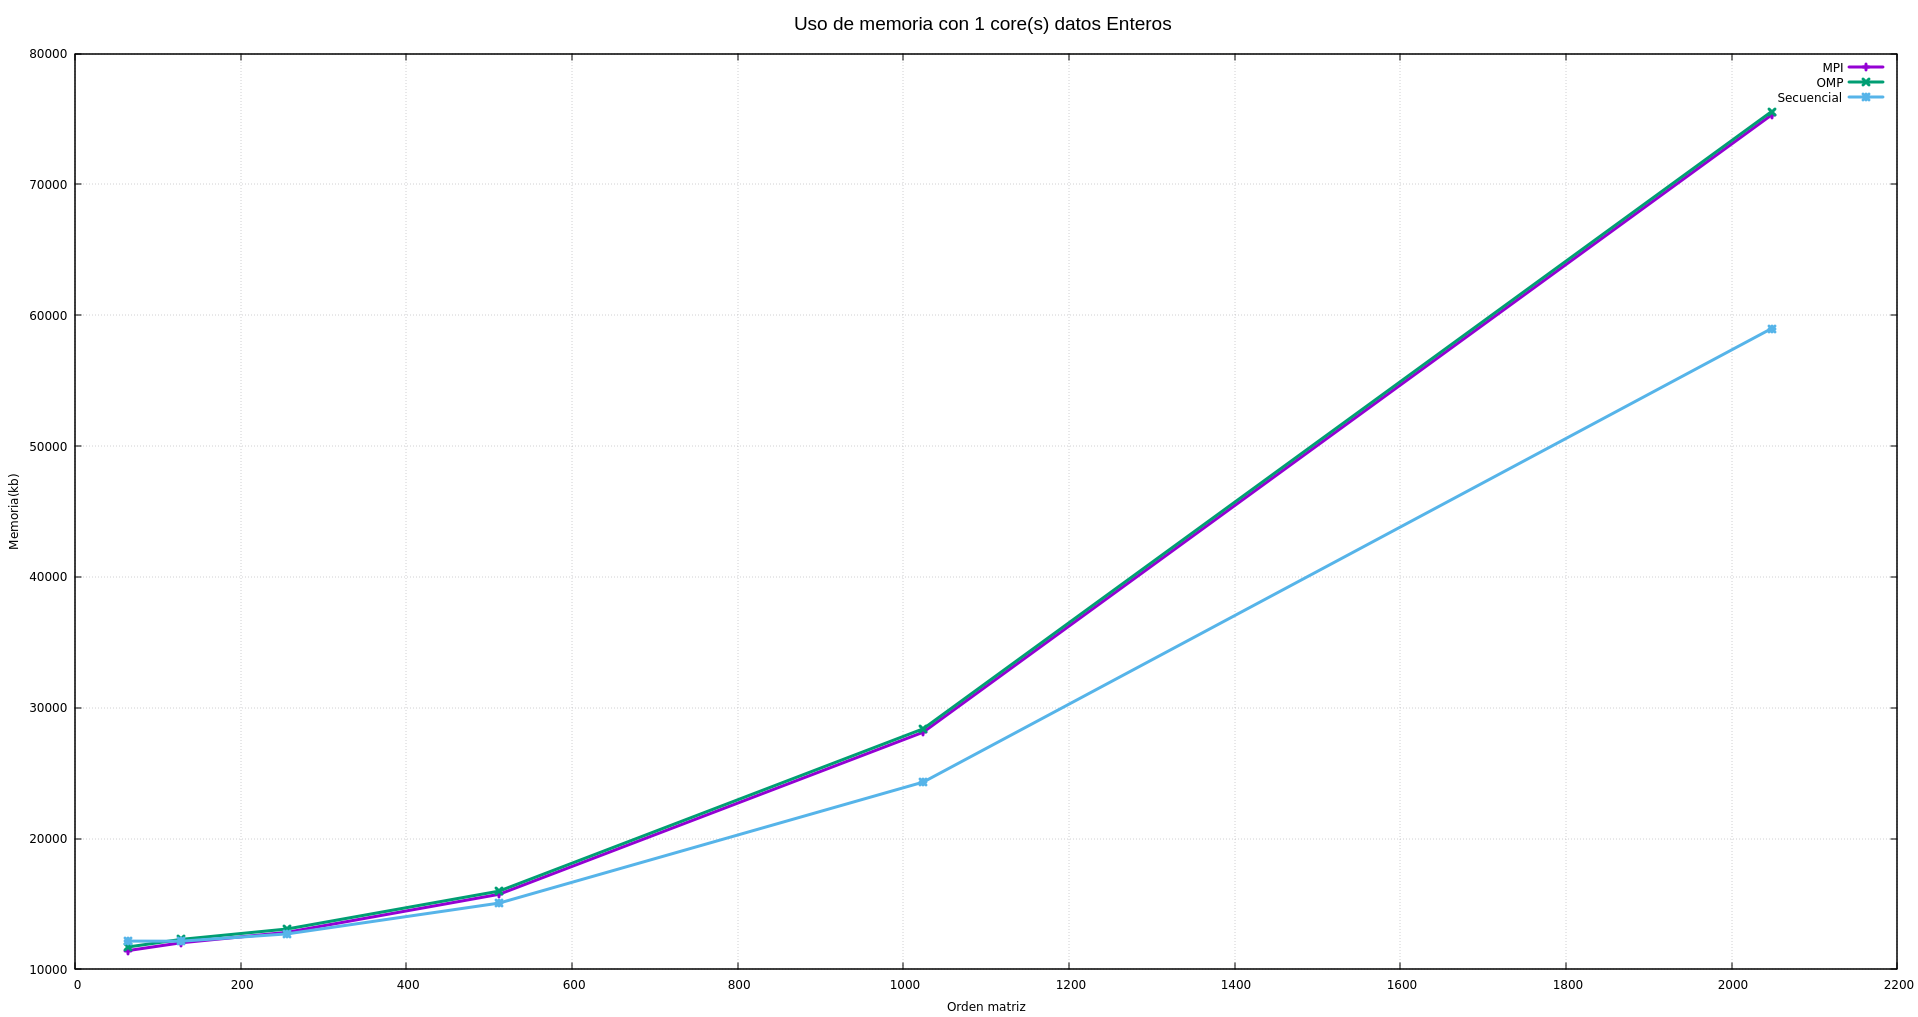
\includegraphics[width=0.95\linewidth]{figs/1nucleoEnterosMemoria.png}
  \caption{Uso de memoria(kb) datos Int 1 cores}
  \label{fig:int2}
\end{figure}

\begin{table}[H]
  \caption{Uso de memoria(kb) datos Int 1 cores}
  \label{table_example}
  \centering
  \begin{tabular}{|c|c|c|c|}
    \hline
    \textbf{Orden} & \textbf{MPI} & \textbf{OMP} & \textbf{Secuencial} \\
    \hline
    64 & 11438.880000 & 11714.400000 & 12165.920000 \\
    128 & 12036.120000 & 12291.760000 & 12152.640000 \\
    256 & 12836.840000 & 13084.960000 & 12711.640000 \\
    512 & 15736.800000 & 15980.560000 & 15066.280000 \\
    1024 & 28129.320000 & 28386.360000 & 24315.680000 \\
    2048 & 75296.280000 & 75557.976992 & 58971.680000 \\
    \hline
  \end{tabular}
\end{table}

\subsection{Resultados con 4 nucleos}

\begin{figure}[H]
  \centering
  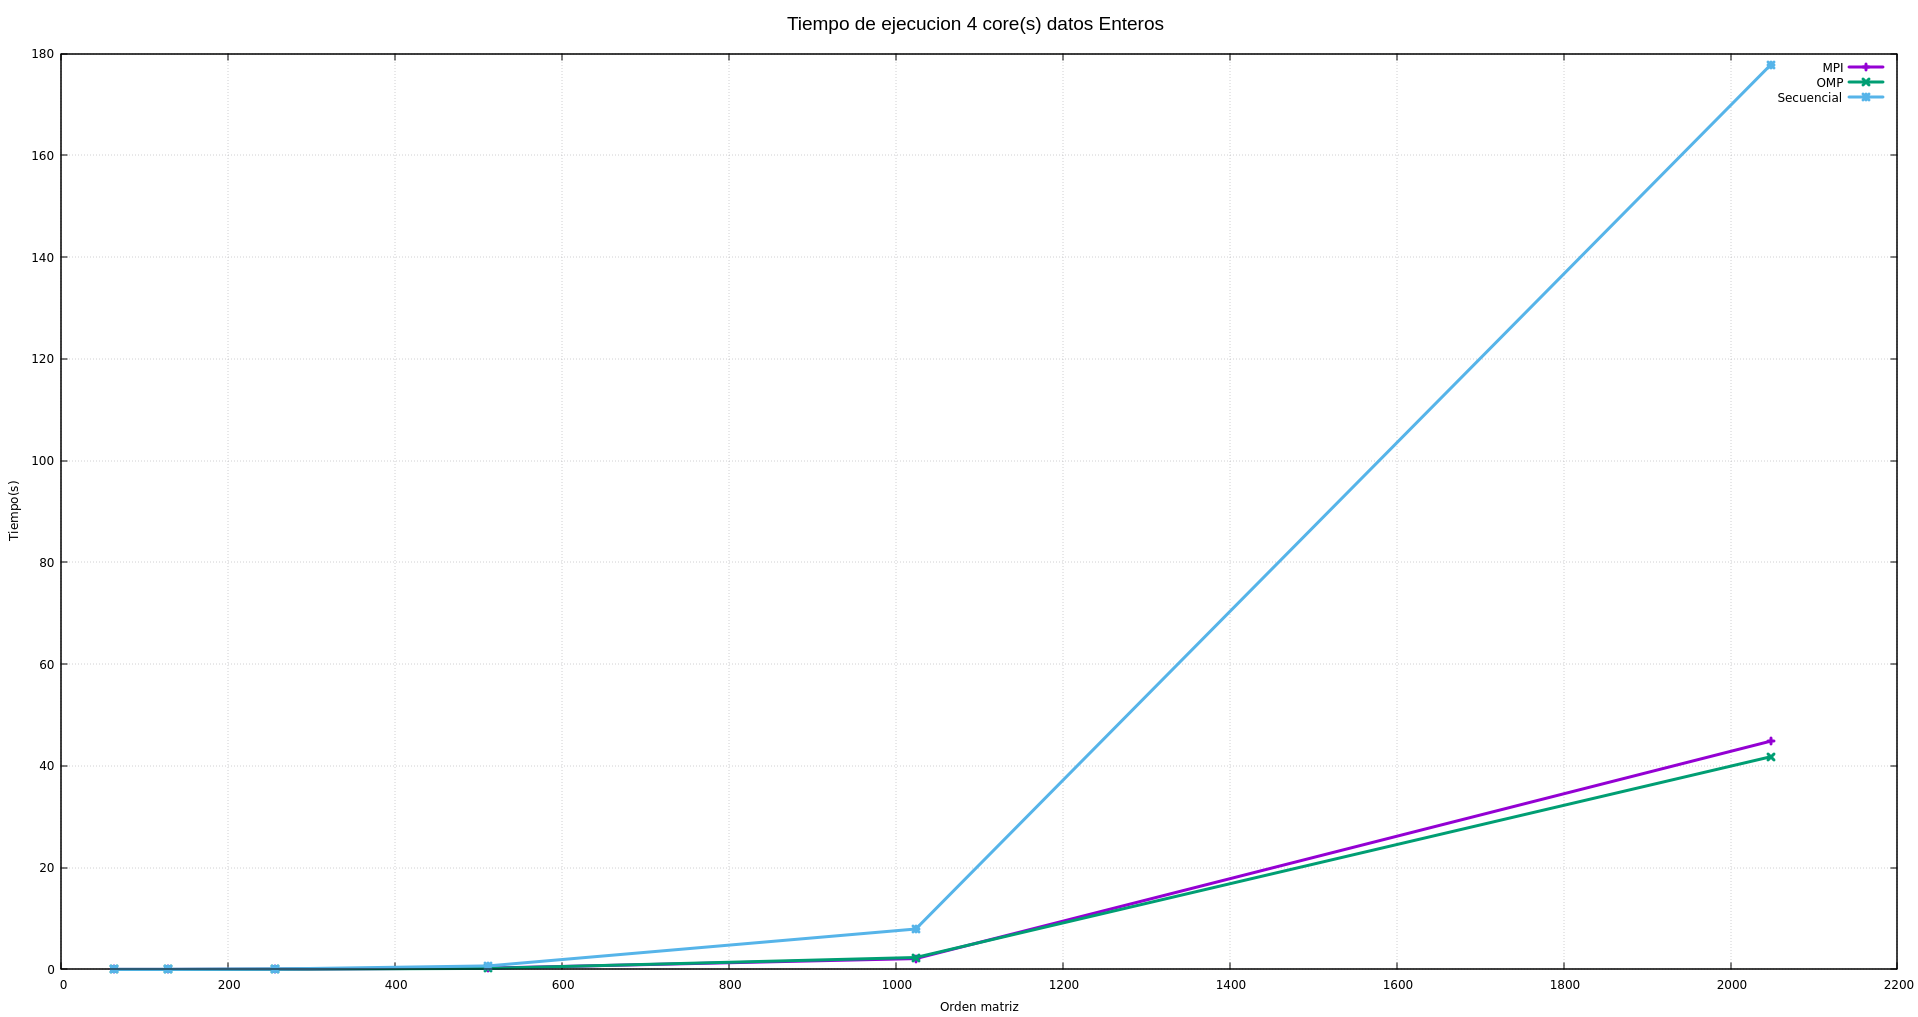
\includegraphics[width=0.95\linewidth]{figs/4nucleosEnterosTiempo.png}
  \caption{Tiempo de ejecución datos Int 4 nucleo}
  \label{fig:in}
\end{figure}

\begin{table}[H]
  \caption{Tiempo de ejecución datos Int 4 nucleo}
  \label{table_example}
  \centering
  \begin{tabular}{|c|c|c|c|}
    \hline
    \textbf{Orden} & \textbf{MPI} & \textbf{OMP} & \textbf{Secuencial} \\
    \hline
    64 & 0.000862 & 0.000735 & 0.000924 \\
    128 & 0.005727 & 0.004896 & 0.008235 \\
    256 & 0.036673 & 0.032910 & 0.080314 \\
    512 & 0.257365 & 0.204609 & 0.693803 \\
    1024 & 2.114608 & 2.339536 & 7.939406 \\
    2048 & 44.848536 & 41.772330 & 177.748948 \\
    \hline
  \end{tabular}
\end{table}

\begin{figure}[H]
  \centering
  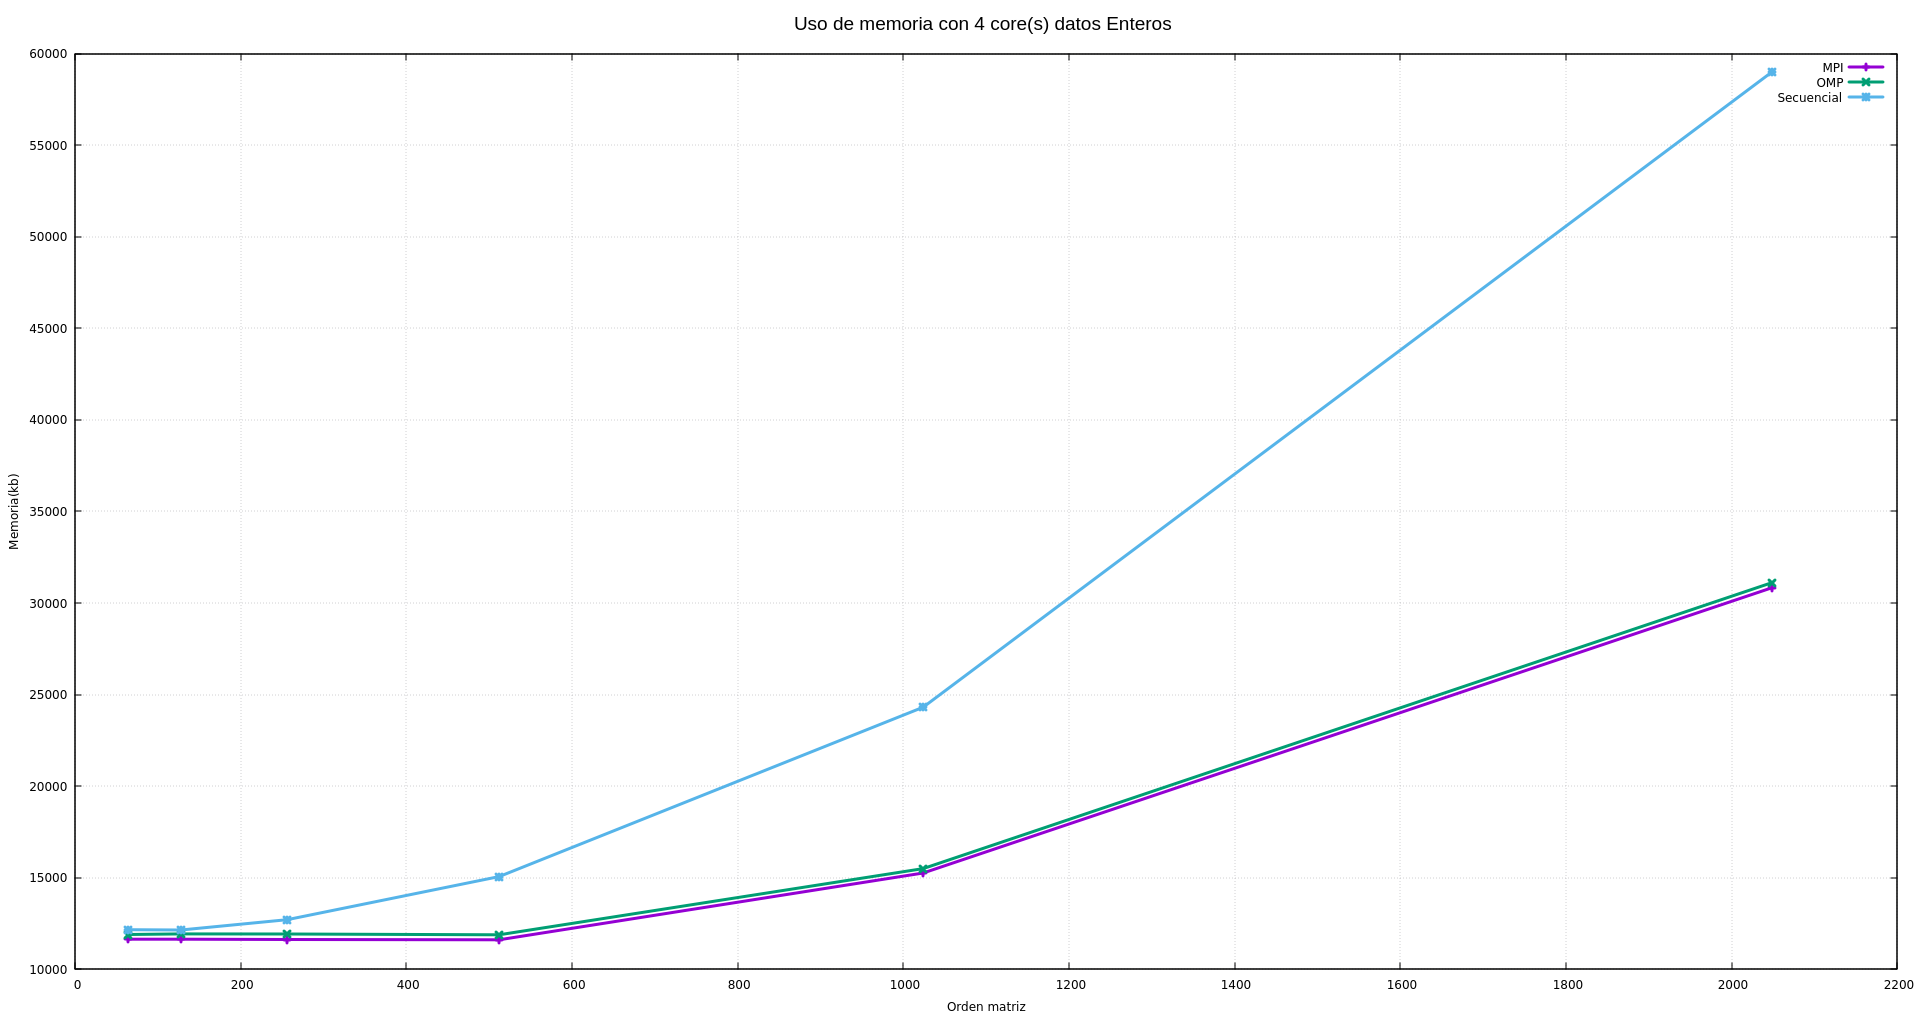
\includegraphics[width=0.95\linewidth]{figs/4nucleosEnterosMemoria.png}
  \caption{Uso de memoria(kb) datos Int 4 cores}
  \label{fig:in2}
\end{figure}

\begin{table}[H]
  \caption{Uso de memoria(kb) datos Int 4 cores}
  \label{table_example}
  \centering
  \begin{tabular}{|c|c|c|c|}
    \hline
    \textbf{Orden} & \textbf{MPI} & \textbf{OMP} & \textbf{Secuencial} \\
    \hline
    64 & 11649.920000 & 11905.240000 & 12165.920000 \\
    128 & 11650.720000 & 11937.160000 & 12152.640000 \\
    256 & 11634.440000 & 11932.040000 & 12711.640000 \\
    512 & 11616.680000 & 11891.040000 & 15066.280000 \\
    1024 & 15264.320000 & 15501.040000 & 24315.680000 \\
    2048 & 30827.120000 & 31107.600000 & 58971.680000 \\
    \hline
  \end{tabular}
\end{table}

\subsection{Datos Float}

\subsection{Resultados con un nucleo}

\begin{figure}[H]
  \centering
  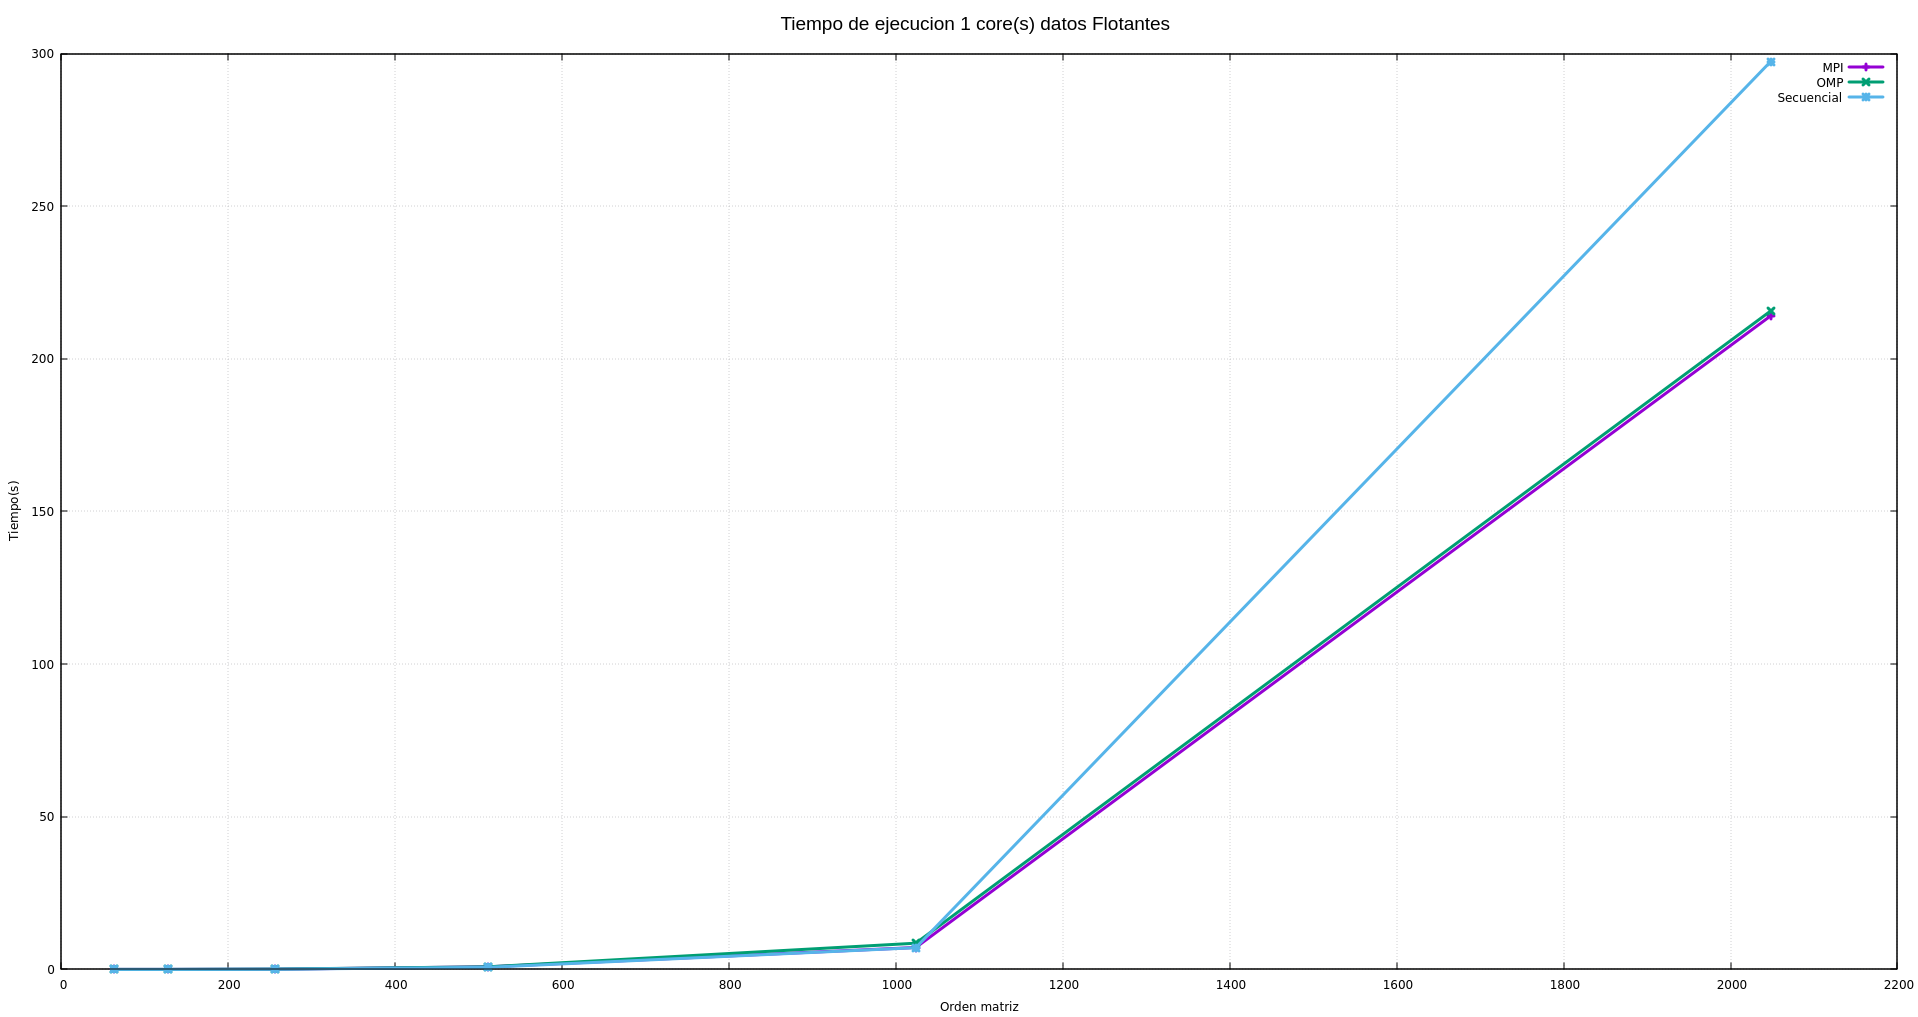
\includegraphics[width=0.95\linewidth]{figs/1nucleoFlotantesTiempo.png}
  \caption{Tiempo de ejecución datos Float 1 nucleo}
  \label{fig:flo}
\end{figure}

\begin{table}[H]
  \caption{Tiempo de ejecución datos Float 1 nucleo}
  \label{table_example}
  \centering
  \begin{tabular}{|c|c|c|c|}
    \hline
    \textbf{Orden} & \textbf{MPI} & \textbf{OMP} & \textbf{Secuencial} \\
    \hline
    64 & 0.001489 & 0.001703 & 0.000943 \\
    128 & 0.012890 & 0.012630 & 0.008589 \\
    256 & 0.071502 & 0.082166 & 0.070707 \\
    512 & 0.841592 & 0.856403 & 0.701360 \\
    1024 & 7.166590 & 8.593199 & 7.119998 \\
    2048 & 214.007155 & 215.613570 & 297.314756 \\
    \hline
  \end{tabular}
\end{table}

\begin{figure}[H]
  \centering
  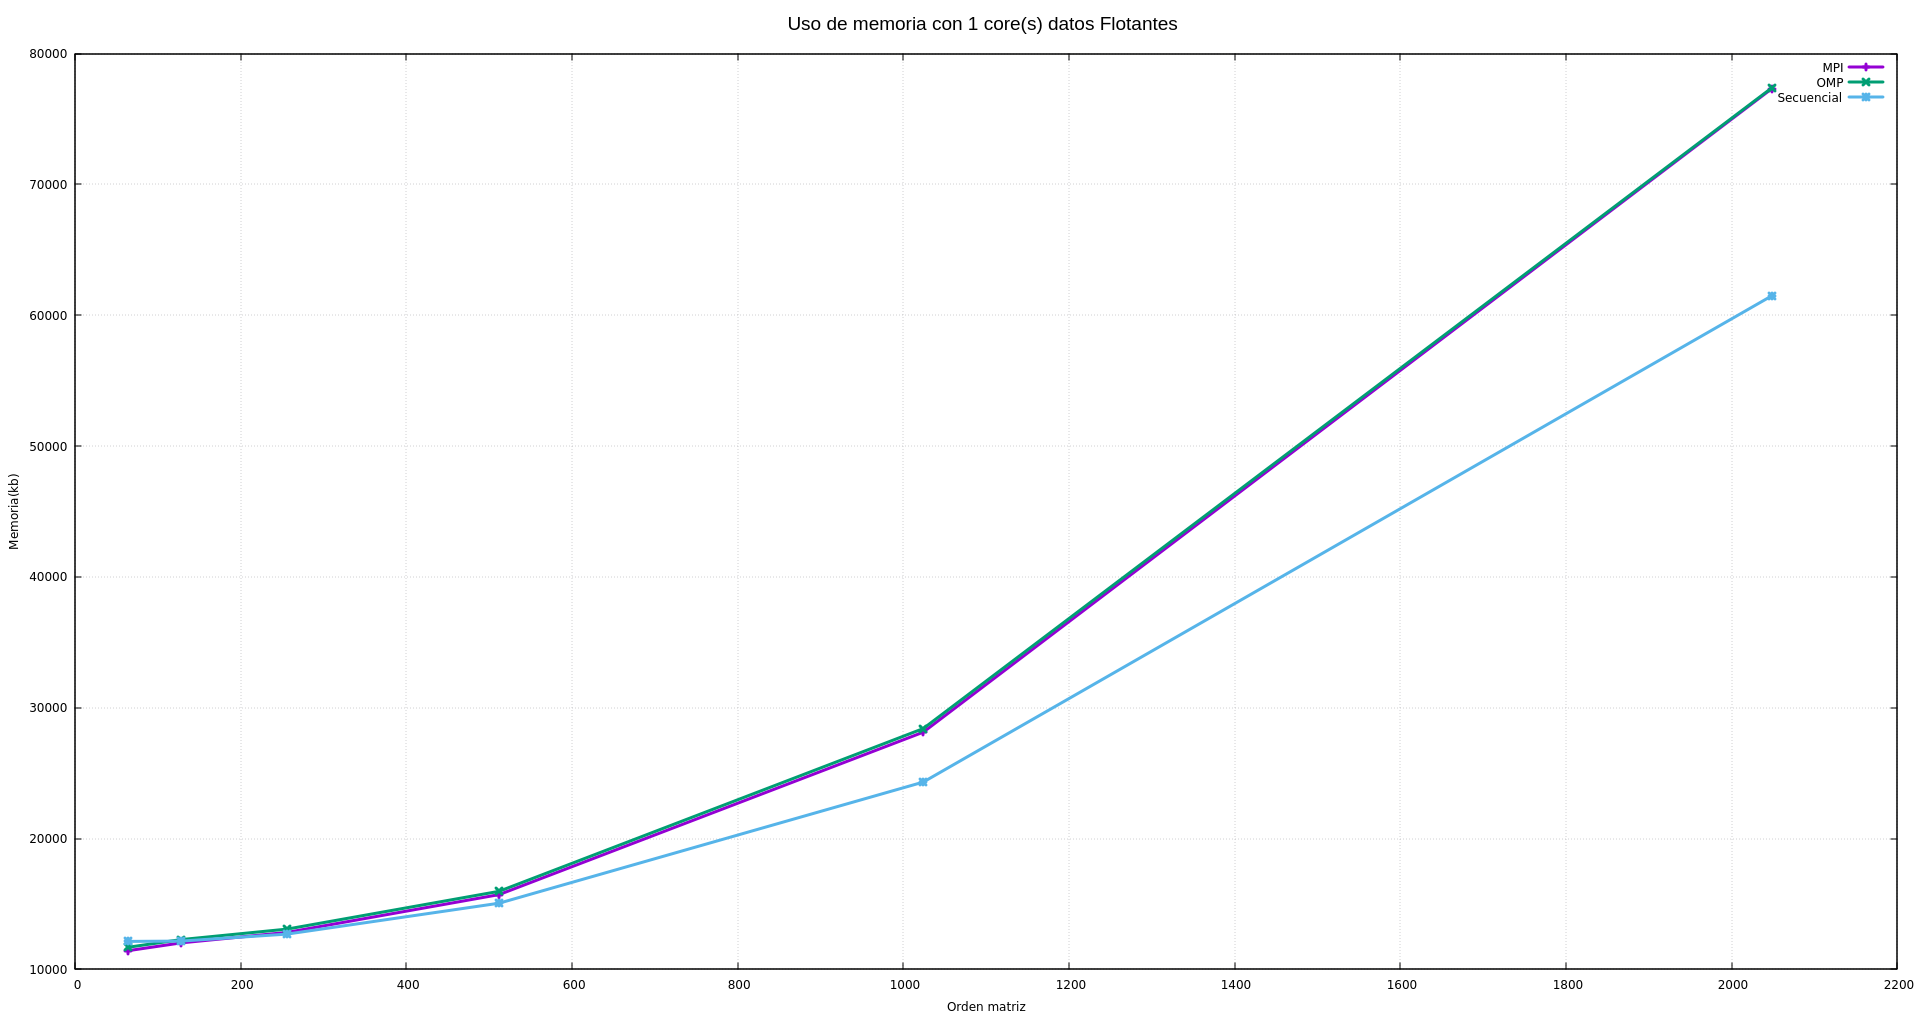
\includegraphics[width=0.95\linewidth]{figs/1nucleoFlotantesMemoria.png}
  \caption{Uso de memoria(kb) datos Float 1 cores}
  \label{fig:flo2}
\end{figure}

\begin{table}[H]
  \caption{Uso de memoria(kb) datos Float 1 cores}
  \label{table_example}
  \centering
  \begin{tabular}{|c|c|c|c|}
    \hline
    \textbf{Orden} & \textbf{MPI} & \textbf{OMP} & \textbf{Secuencial} \\
    \hline
    64 & 11431.240000 & 11687.280000 & 12139.880000 \\
    128 & 12025.200000 & 12279.520000 & 12159.520000 \\
    256 & 12827.120000 & 13079.760000 & 12699.120000 \\
    512 & 15716.120000 & 15972.040000 & 15059.160000 \\
    1024 & 28129.160000 & 28401.400000 & 24313.360000 \\
    2048 & 77297.944431 & 77352.005185 & 61469.240000 \\
    \hline
  \end{tabular}
\end{table}

\subsection{Resultados con 4 nucleos}

\begin{figure}[H]
  \centering
  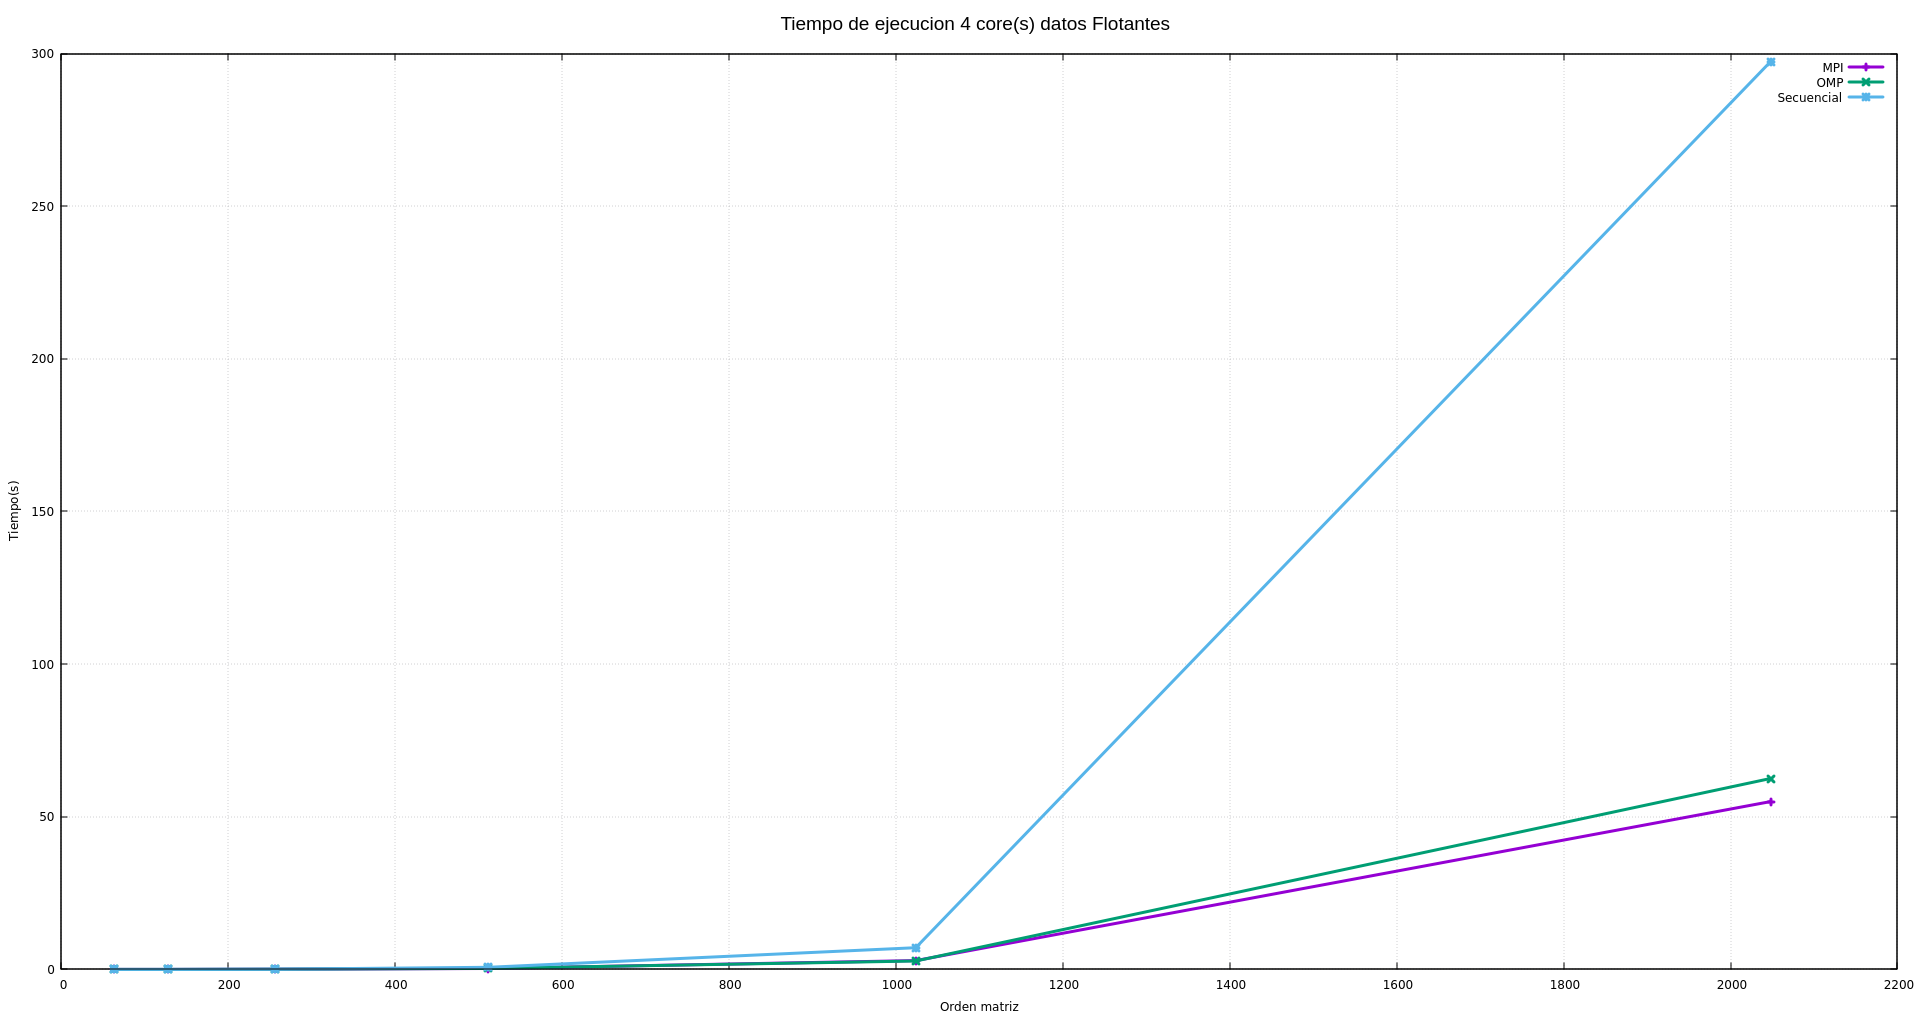
\includegraphics[width=0.95\linewidth]{figs/4nucleosFlotantesTiempo.png}
  \caption{Tiempo de ejecución datos Float 4 nucleo}
  \label{fig:f}
\end{figure}

\begin{table}[H]
  \caption{Tiempo de ejecución datos Float 4 nucleo}
  \label{table_example}
  \centering
  \begin{tabular}{|c|c|c|c|}
    \hline
    \textbf{Orden} & \textbf{MPI} & \textbf{OMP} & \textbf{Secuencial} \\
    \hline
    64 & 0.001141 & 0.001212 & 0.000943 \\
    128 & 0.006673 & 0.007279 & 0.008589 \\
    256 & 0.072421 & 0.071444 & 0.070707 \\
    512 & 0.311020 & 0.315073 & 0.701360 \\
    1024 & 2.871131 & 2.762083 & 7.119998 \\
    2048 & 54.975360 & 62.538980 & 297.314756 \\
    \hline
  \end{tabular}
\end{table}

\begin{figure}[H]
  \centering
  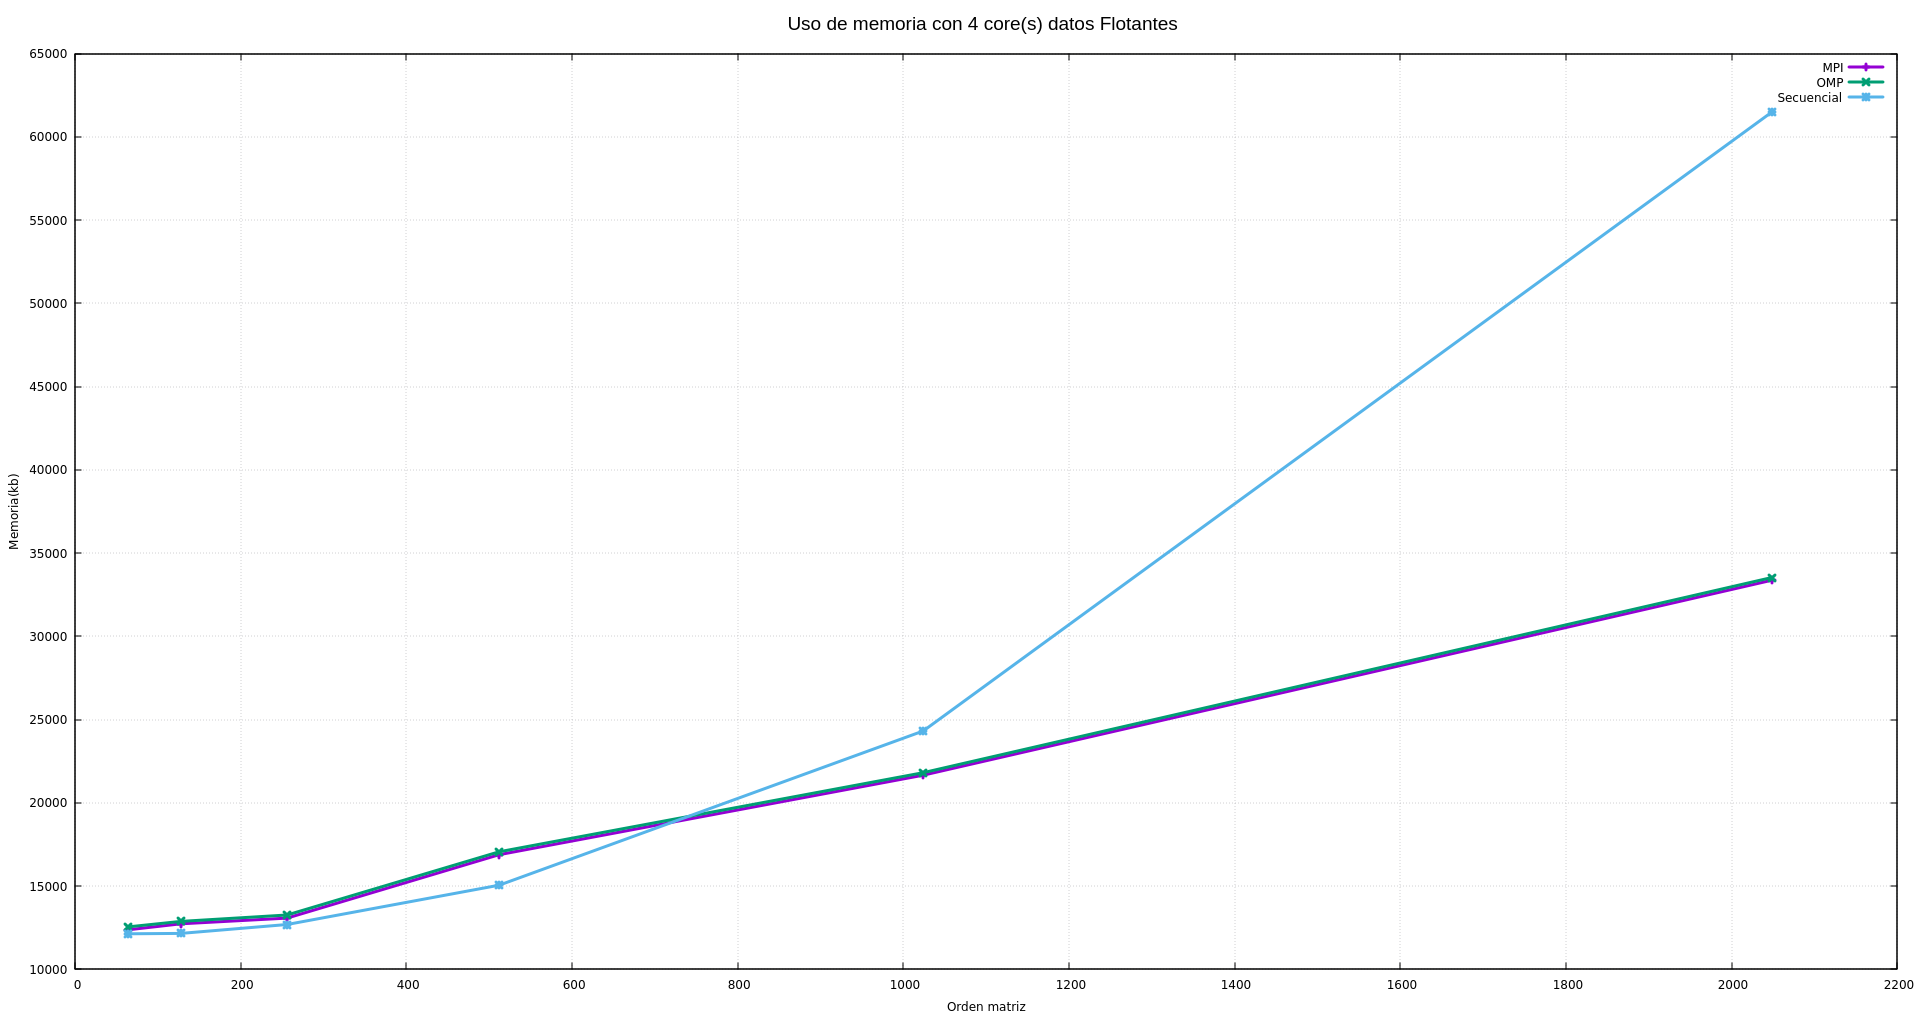
\includegraphics[width=0.95\linewidth]{figs/4nucleosFlotantesMemoria.png}
  \caption{Uso de memoria(kb) datos Float 4 cores}
  \label{fig:f2}
\end{figure}

\begin{table}[H]
  \caption{Uso de memoria(kb) datos Float 4 cores}
  \label{table_example}
  \centering
  \begin{tabular}{|c|c|c|c|}
    \hline
    \textbf{Orden} & \textbf{MPI} & \textbf{OMP} & \textbf{Secuencial} \\
    \hline
    64 & 12376.520000 & 12551.040000 & 12139.880000 \\
    128 & 12738.760000 & 12883.240000 & 12159.520000 \\
    256 & 13080.080000 & 13266.720000 & 12699.120000 \\
    512 & 16886.000000 & 17063.000000 & 15059.160000 \\
    1024 & 21664.040000 & 21812.280000 & 24313.360000 \\
    2048 & 33367.840000 & 33525.840000 & 61469.240000 \\
    \hline
  \end{tabular}
\end{table}

\subsection{Datos Doubles}

\subsection{Resultados con un nucleo}

\begin{figure}[H]
  \centering
  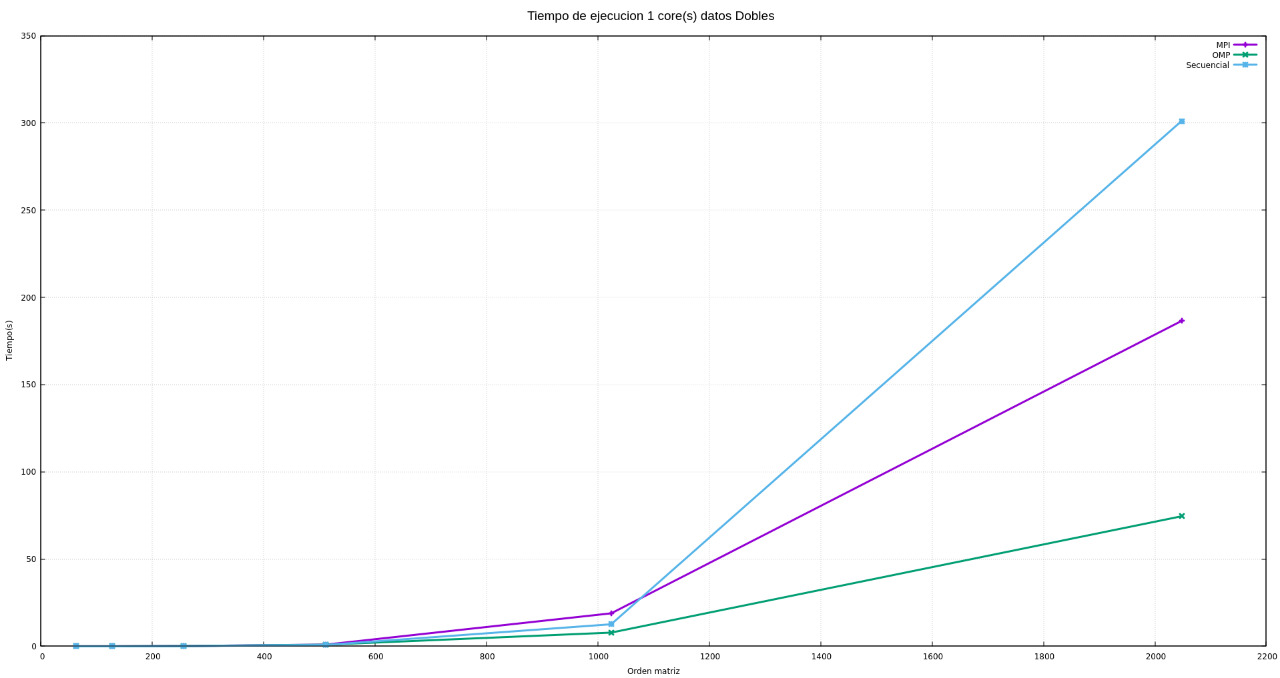
\includegraphics[width=0.95\linewidth]{figs/1nucleoDoblesTiempo.jpeg}
  \caption{Tiempo de ejecución datos Doubles 1 nucleo}
  \label{fig:do}
\end{figure}

\begin{table}[H]
  \caption{Tiempo de ejecución datos Doubles 1 nucleo}
  \label{table_example}
  \centering
  \begin{tabular}{|c|c|c|c|}
    \hline
    \textbf{Orden} & \textbf{MPI} & \textbf{OMP} & \textbf{Secuencial} \\
    \hline
    64 & 0.001572 & 0.001734 & 0.000959 \\
    128 & 0.010962 & 0.013741 & 0.008877 \\
    256 & 0.106090 & 0.107374 & 0.091583 \\
    512 & 0.937029 & 0.915204 & 0.763535 \\
    1024 & 18.874105 & 7.816300 & 12.601943 \\
    2048 & 186.494606 & 74.509577 & 301.081461 \\
    \hline
  \end{tabular}
\end{table}

\begin{figure}[H]
  \centering
  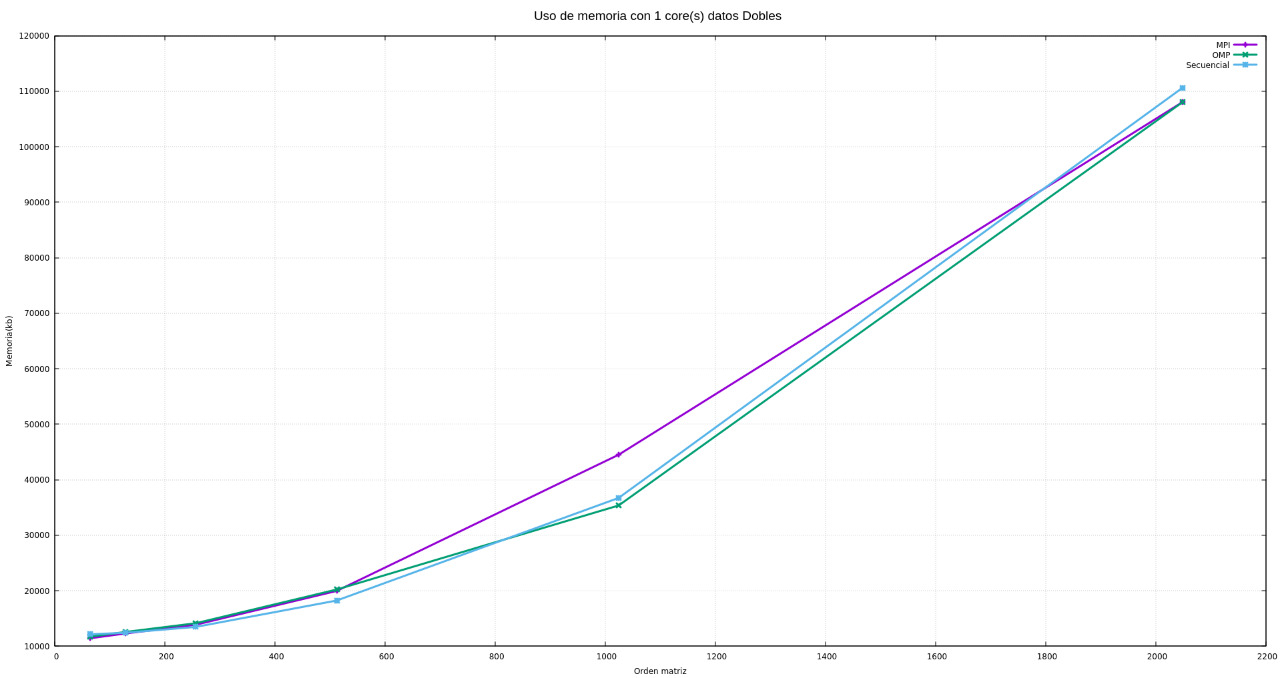
\includegraphics[width=0.95\linewidth]{figs/1nucleoDoblesMemoria.jpeg}
  \caption{Uso de memoria(kb) datos Double 1 cores}
  \label{fig:do2}
\end{figure}

\begin{table}[H]
  \caption{Uso de memoria(kb) datos Double 1 cores}
  \label{table_example}
  \centering
  \begin{tabular}{|c|c|c|c|}
    \hline
    \textbf{Orden} & \textbf{MPI} & \textbf{OMP} & \textbf{Secuencial} \\
    \hline
    64 & 11446.040000 & 11716.360000 & 12161.306931 \\
    128 & 12296.560000 & 12570.080000 & 12420.160000 \\
    256 & 13878.640000 & 14139.160000 & 13485.360000 \\
    512 & 19973.240000 & 20215.160000 & 18235.760000 \\
    1024 & 44503.120000 & 35371.135802 & 36723.400000 \\
    2048 & 108042.880000 & 108027.520000 & 110616.200000 \\
    \hline
  \end{tabular}
\end{table}

\subsection{Resultados con 4 nucleos}

\begin{figure}[H]
  \centering
  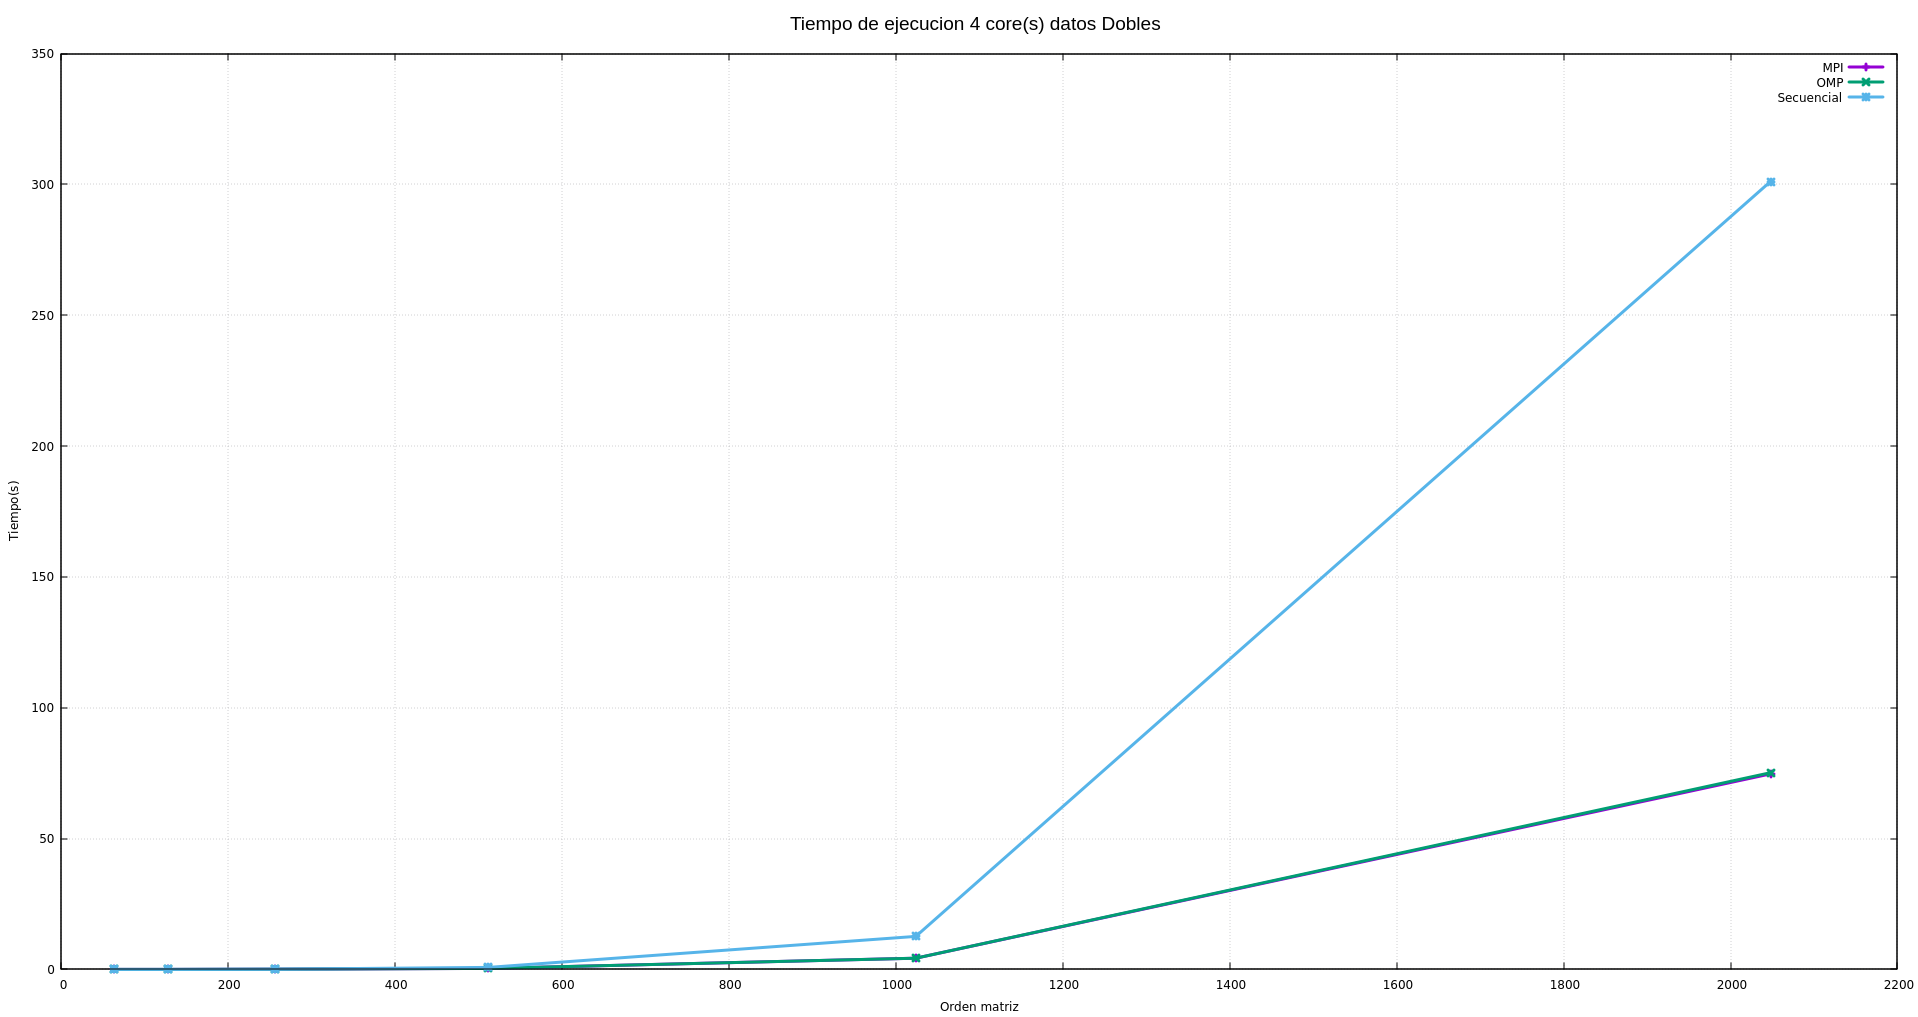
\includegraphics[width=0.95\linewidth]{figs/4nucleosDoblesTiempo.png}
  \caption{Tiempo de ejecución datos Doubles 4 nucleo}
  \label{fig:d}
\end{figure}

\begin{table}[H]
  \caption{Tiempo de ejecución datos Doubles 4 nucleo}
  \label{table_example}
  \centering
  \begin{tabular}{|c|c|c|c|}
    \hline
    \textbf{Orden} & \textbf{MPI} & \textbf{OMP} & \textbf{Secuencial} \\
    \hline
    64 & 0.001501 & 0.001280 & 0.000959 \\
    128 & 0.007319 & 0.006673 & 0.008877 \\
    256 & 0.073958 & 0.079893 & 0.091583 \\
    512 & 0.393405 & 0.380872 & 0.763535 \\
    1024 & 4.281900 & 4.283746 & 12.601943 \\
    2048 & 74.692427 & 75.154596 & 301.081461 \\
    \hline
  \end{tabular}
\end{table}

\begin{figure}[H]
  \centering
  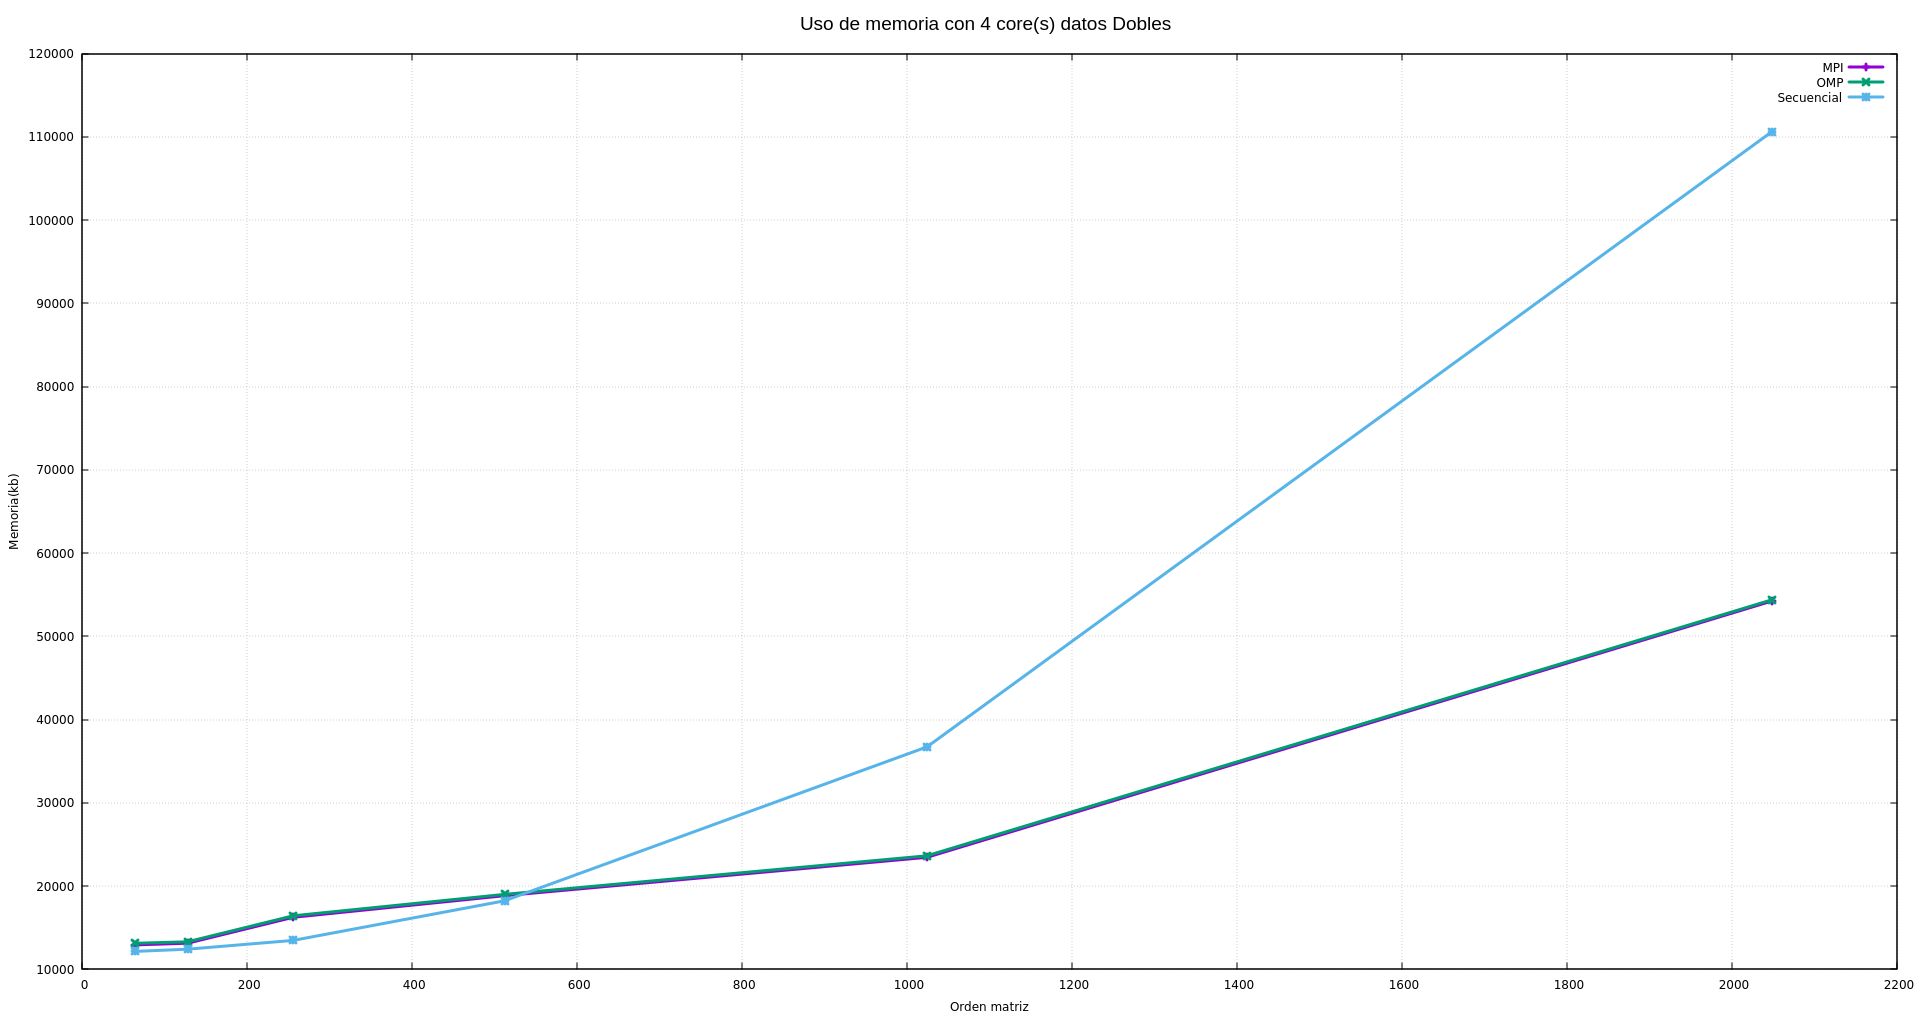
\includegraphics[width=0.95\linewidth]{figs/4nucleosDoblesMemoria.png}
  \caption{Uso de memoria(kb) datos Double 4 cores}
  \label{fig:d2}
\end{figure}

\begin{table}[H]
  \caption{Uso de memoria(kb) datos Double 4 cores}
  \label{table_example}
  \centering
  \begin{tabular}{|c|c|c|c|}
    \hline
    \textbf{Orden} & \textbf{MPI} & \textbf{OMP} & \textbf{Secuencial} \\
    \hline
    64 & 12944.000000 & 13135.640000 & 12161.306931 \\
    128 & 13146.680000 & 13311.760000 & 12420.160000 \\
    256 & 16252.400000 & 16440.680000 & 13485.360000 \\
    512 & 18852.440000 & 19012.600000 & 18235.760000 \\
    1024 & 23466.640000 & 23638.040000 & 36723.400000 \\
    2048 & 54244.080000 & 54393.400000 & 110616.200000 \\
    \hline
  \end{tabular}
\end{table}

\section{Conclusiones}
Las evidencias sugieren un mejor funcionamiento por parte de los algoritmos secuenciales durante la multiplicación de matrices pequeñas, sin embargo nos percatamos de la desventaja en todo sentido durante el incremento del orden. Durante el desarrollo de resultados también es notoria la diferencia en el tiempo de ejecución pues lo que a los algoritmos secuenciales les tomaría más de dos horas cuando hablamos de orden 2048 , los algoritmos en FOX MPI o OMP amplían el margen pues terminan sus resultados en menos de una hora, el uso de Memoria es especialmente relevante puesto que al momento de correr los algoritmos se ralentiza la velocidad en la computadora y no es posible realizar otras actividades hasta el término de estos, lógicamente en los algoritmos secuenciales esto se acentúa y en los paralelos es más difícil de distinguir. Al aplicar estos tipos de datos durante la ejecución inferimos los datos enteros y flotantes se mantienen en un tiempo promedio  de ambos. Esto debido al tamaño que se maneja en el lenguaje C correspondiente en números de bytes. Para finalizar es importante destacar que es un trabajo el cual nos lleva al correcto entendimiento de las ventajas de los algoritmos Fox En paralelo sobre los secuenciales así como varias de las aplicaciones que tiene la programación paralela en los sistemas de manejo de grandes volúmenes de datos.

\section{Referencias}
{[1]} Fox G., M. Johnson, G. Lyzenga, S. Otto, J. Salmon, and D. Walker, Solving Problems on Concurrent Processors, Vol. I, Prentice Hall, Englewood Cliffs, New Jersey, 1988.
{[2]} Choi J., J. Dongarra, D. Walker, PUMMA: Parallel Universal Matrix Multiplication Algorithm on Distributed Memory Concurrent Computers, in Concurrency: Practice and Experience, 6:543-570,2007.

\end{document}
